\newcommand{\lc}{LC\xspace}
\newcommand{\prc}{PR\xspace}
\newcommand{\smc}{SMC\xspace}
\newcommand{\kcore}{k_{core}}
\newcommand{\kmesh}{k_{mesh}}
\newcommand{\kram}{k_{ram}}

\lstset{
language=C,
numbers=left,
numberstyle=\footnotesize,
frame=single}

\lstset{deletekeywords={bool,int}}
\lstset{morekeywords={foreach,in}}

\lstset{classoffset=1, morekeywords={ZERO,ONE,LOCAL\_MANY,GLOBAL,FORWARDED},keywordstyle=\color{Red},
        classoffset=2, morekeywords={pointer,bool,int,Val,Ref,ThreadID,Thread,Set},keywordstyle=\color{OliveGreen}, %Types
        classoffset=0}% restore default


\chapter{\MMSCC: A Coherent and Managed Runtime for ML on the SCC}
\label{chap:aneris}

In this chapter, we describe \MMSCC, an extension of \MM that provides a
coherent address space on the SCC, optimizing for the SCC's memory hierarchy.
We begin with a \emph{local collector}\footnote{Other terms have been used in
the literature to indicate similar heap designs, notably private nursery, local
heap collector, thread-local or thread-specific heap, and on-the-fly
collection.} (\lc)
design~\cite{Steele75,Doligez93,Steensgaard00,Anderson10,Marlow11,Auhagen11}
that partitions the heap into local heaps on each core and a shared heap for
cross-core communication. However, we observe that the cost of memory barriers
utilized in preserving the heap invariants have significant costs. To
eliminitate theses costs, we propose a new GC design (\prc) that utilizes the
ample concurrency offered by our programming model combined with a dynamic
shape analysis to eliminate some of the GC overheads. This naturally leads to a
GC design that focuses on \emph{procrastination}~\cite{mmgc}, delaying writes
that would necessitate establishing forwarding pointers until a GC, where there
is no longer a need for such pointers. The GC leverages the mostly functional
nature of ACML programs and a new object property called \emph{cleanliness},
which enables a broad class of objects to be moved from a local to a shared
heap without requiring a full traversal of the local heap to fix existing
references; cleanliness enables an important optimization that achieves the
effect of procrastination without actually having to initiate a thread stall.
Our final design (\smc) integrates SCC's support for software-managed cache
coherence (SMC)~\cite{SMC} into the extant memory barriers to improve the
design further.

We begin by discussing in detail the architecture and programming model of the
SCC, which serves as our prototype non cache coherent architecture. However,
the use of SCC by no means restricts the applicability of our ideas to other
scalable manycore architectures~\cite{mmgc}. Then, we present the three GC
designs. Finally, we present a comprehensive evaluation of the three designs.

\section{The Intel Single-chip Cloud Computer}

\begin{figure}
\begin{center}
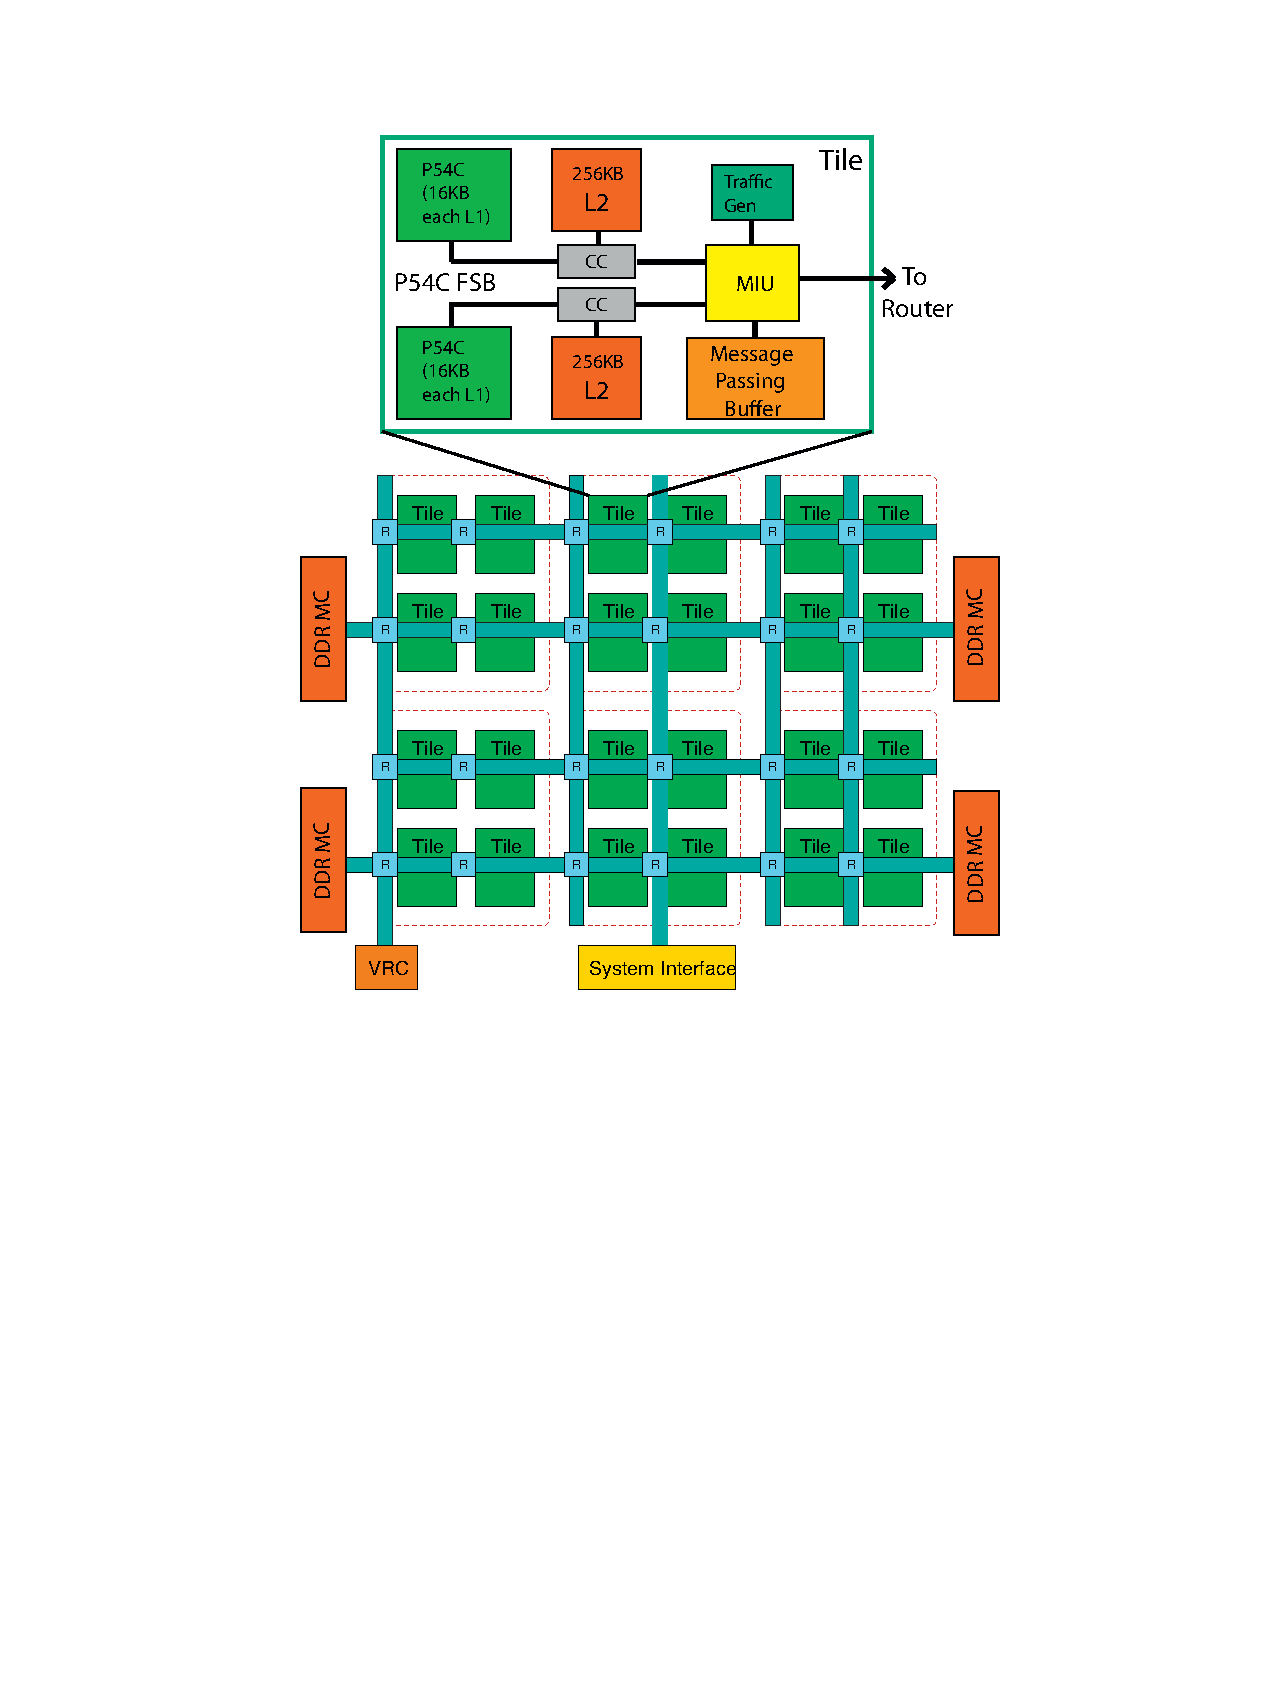
\includegraphics{Figures/SCC.pdf}
\end{center}
\caption{The architecture of the Intel SCC processor}
\label{fig:scc}
\end{figure}

Intel SCC~\cite{Mattson2010} (Figure~\ref{fig:scc}) is a many-core processor
with 48 P54C cores on a single chip, grouped as 24 tiles, organized in a 4
$\times$ 6 mesh network with a bisection bandwidth of 256 Gb/s. The most
interesting aspect of the SCC architecure is the complete lack of cache
coherence between the cores, and the presence of fast on-die message-passing
network interface. The 24 tiles on the chip are divinded into 4 quadrants, and
each quadrant is connected to a DDR3 memory controller. Each core has 16KB of
private L1 instruction and data caches, and 256 KB of L2 cache shared with the
other core on the same tile.

In addition, each tile has a 16KB message-passing buffer (MPB) used for
message-passing between the cores. The message passing buffers are the only
caches that are accessible across all of the cores. The data used in on-chip
communication is read from MPB, cached in L1 cache, but bypasses the L2 cache.
The cache uses no-allocate policy on writes, and L1 cache incorporates a
write-combine buffer. According to the processor
specifications~\cite{Mattson2010}, the read latencies in this architecure are:
\begin{mathpar}
\begin{array}{rcl}
\textrm{LocalMPB} & = & 45~\kcore + 8~\kmesh \\
\textrm{RemoteMPB} & = & 45~\kcore + 4*n*2~\kmesh \\
\textrm{DRAM} & = & 40~\kcore + 4*n*2~\kmesh + 46~\kram
\end{array}
\end{mathpar}

\noindent where $\kcore$, $\kmesh$ and $\kram$ are the cycles of core, mesh
network and memory respectively. In our experimental setup, where 6 tiles share
a memory controller, the number of hops n to the memory controller could be $0
< n \le 8$. Hence, the DRAM accesses are far more expensive than the MPBs. Each
core additionally has a test and set register that is accessible from all other
cores. The SCC uses 32-bit Pentium cores. A programmable, software-managed
Look-Up Table (LUT) provides a means for implementing hybrid private and shared
address spaces in the system.

\subsection{Software System}

From the programmer's point of view, SCC resembles a cluster of nodes, with
portions of memory shared between the cores. Each core runs a linux kernel
image, and does not share any operating system services with the other cores.
Since SCC does not provide harware cache coherence, it provides software
support for managing coherence. First, SCC provides support for tagging a
specific virtual address space as shared across all of the cores. Caching can
also be selectively enabled on this address space; SCC tags this address space
as having message passing buffer type (MPBT).

Data typed as MPBT bypass L2 and go directly to L1. SCC also provides a
special, 1-cycle instruction called \cf{CL1INVMB} that marks all data of type
MPBT as invalid L1 lines. In addition, the usual \cf{WBINVD} instruction can be
used to flush and invalidate the L1 cache. Since the cores use write-combine
buffers, a correct flushing procedure should also flush the write-combine
buffers. SCC does not provide primitive support for this purpose, but
write-combine buffers can easily be flushed in software by perfoming a series
of dummy writes to distinct memory locations, which fills the buffer and
flushes any previous writes.

Typically, a programmer works with release consistency in order to utilize
cached shared virtual memory. The SMC~\cite{SMC} library provides
\cf{smcAcquire()} to fetch changes from other cores (invalidates MPBT cache
lines in L1 cache) and issues \cf{smcRelease()} to publish its updates (flushes
the L1 cache, if the cache is operating in write back mode, and flushes the
write-combine buffers).

SCC's software stack also includes cross-core message-passing libraries
implemented over the MPBs, including RCCE~\cite{Mattson2010} and
RCKMPI~\cite{Urena2011}. RCCE is optimized for Single Program Multiple Data
(SPMD) parallel programming model, where the program is structured in such a
way that the sender and the receiver ideally arrive at the communication point
at the same time. The sender writes the message to the MPB, while the receiver
busy waits (invalidating its cache every iteration to fetch recent writes),
waiting for a special flag value to be written along with the message. After
the sender writes the flag, the receiver reads the message into its private
memory, while the sender busy waits (also invalidating its cache every
iteration). Finally, the receiver writes a completion flag, which concludes the
message transfer.

It is worthwhile pointing out that RCCE uses just the MPBs, while RCKMPI uses
MPBs for small messages (less than 8KB --- the maximum message size that would
fully fit in the MPB) and the DRAM for larger messages. Despite having a higher
bandwidth and lower latency, the synchronization costs involved in transferring
a large multi-part message over the MPB overweighs the benefits.

\section{Local Collector (\lc)}
\label{sec:lc}

Splitting a program heap among a set of cores is a useful technique to exploit
available parallelism on scalable multicore platforms: each core can allocate,
collect, and access data locally, moving objects to a global, shared heap only
when they are accessed by threads executing on different cores. This design
allows local heaps to be collected independently, with coordination required
only for global heap collection. In contrast, stop-the-world collectors need a
global synchronization for every collection.

\subsection{Heap Architecture}

\begin{figure}
\centering
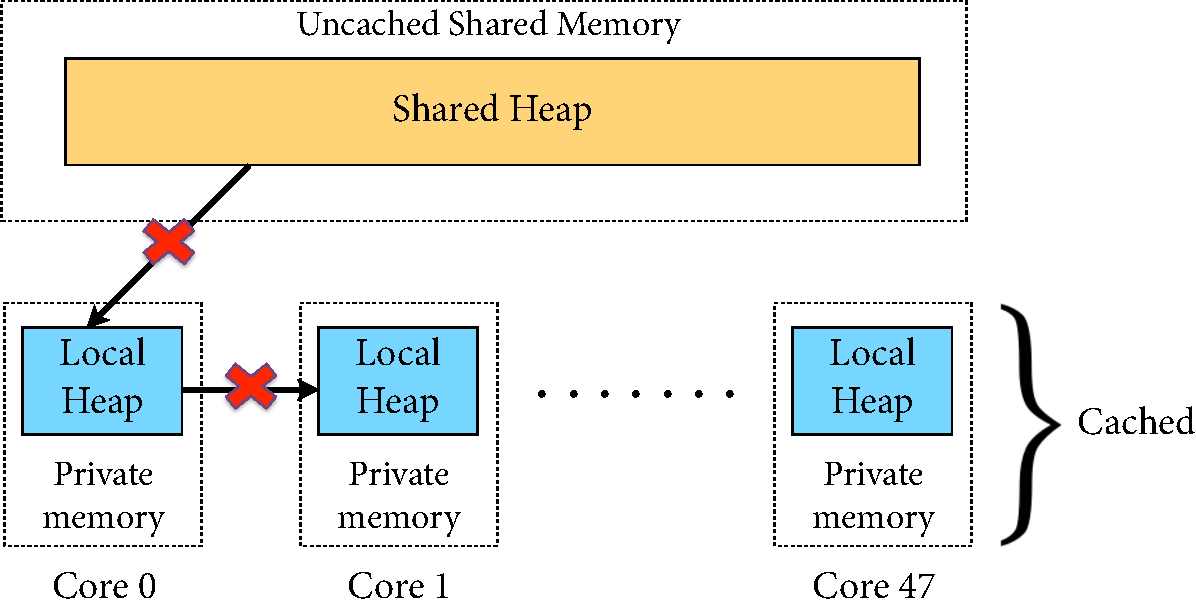
\includegraphics[width=1\textwidth]{Figures/LocalCollector.pdf}
\caption{Local collector heap organization for the SCC}
\label{fig:lc}
\end{figure}


Our local collector design for the SCC is shown in Figure~\ref{fig:lc}. The key
idea here is that the local heaps are allocated in each of the cores
\emph{cached} private memory, into which new objects are allocated by default.
The private heaps are allocated on the memory banks closest to the core to
optimize for the memory hierarchy and reduce mesh congestion. Since the design
allows independent collection of local heaps, the design can scale to hundreds
of cores~\cite{JFP14}, and benefits cache coherent architectures as well. The
shared heap is allocated in the shared memory, and visible to all of the cores.
In order to circumvent the coherence issues, we disable caching on the shared
heap. Hence, every shared memory access goes to the DRAM. The shared heap pages
are interleaved across all of the memory banks to uniformly spread the
requests.

\subsection{Heap Invariants}

In order to ensure that cores cannot directly or indirectly access objects on
other local heaps, which would complicate the ability to perform independent
local heap collection, the following invariants need to be preserved:

\begin{itemize}
\item No pointers are allowed from one core's local heap to another.
\item No pointers are permitted from the shared heap to the local heap.
\end{itemize}

\noindent Both invariants are necessary to perform independent local
collections.  The reason for the first is obvious.  The second invariant
prohibits a local heap from transitively accessing another local heap object
via the shared heap.  In order to preserve these invariants, the mutator
typically executes a \emph{write barrier} on every store operation. The write
barrier ensures that before assigning a local object reference (source) to a
shared heap object (target), the local object along with its transitive object
closure is lifted to the shared heap. We call such writes \emph{exporting
writes} as they export information out of local heaps.  The execution of the
write barrier creates \emph{forwarding pointers} in the original location of
the lifted objects in the local heap. These point to the new locations of the
lifted objects in the shared heap. Since objects can be lifted to the shared
heap on potentially any write, the mutator needs to execute a \emph{read
barrier} on potentially every read. The read barrier checks whether the object
being read is the actual object or a forwarding pointer, and in the latter
case, indirects to the object found on the shared heap.  Forwarding pointers
are eventually eliminated during local collection.

\subsection{Allocation and Collection}

The allocations in the shared heap is performed similar to allocations in the
stop-the-world collector, where each core allocates a page-sized chunk in the
shared heap and performs object allocation by bumping its core-local shared
heap frontier. Allocations in the local heaps do not require any
synchronization. Garbage collection in the local heaps is similar to the
baseline collector, except that it crucially does not require global
synchronization.

Objects are allocated in the shared heap only if they are to be shared between
two or more cores. Objects are automatically lifted to the shared heap because
of exporting writes and spawning a thread on a different core. Apart from
these, all globals are allocated in the shared heap, since globals are visible
to all cores by definition. Thus, for the ML programmer on this system, the
absence of cache coherence is completely hidden, the SCC appears as a cache
coherent multicore machine.

For a shared heap collection, all of the cores synchronize on a barrier and
then a single core collects the heap. Along with globals, all the live
references from local heaps to the shared heap are considered to be roots for a
shared heap collection. In order to eliminate roots from dead local heap
objects, before a shared heap collection, local collections are performed on
each core to eliminate such references.

The shared heap is also collected using Sansom's dual-mode garbage collector.
However, we do not perform generational collection on the shared heap. This is
because of two reasons. First, objects in the shared heap, shared between two
or more cores, are expected to live longer than a typical object collected
during generational collection. Secondly, shared heap collection requires
global synchronization, and it is wise to perform such collections rarely.

\subsection{Remembered stacks}

In \MM threads can synchronously or asynchronously communicate with each other
over first-class message-passing communication channels. If a receiver is not
available, a sender thread, or in the case of asynchronous communication the
implicitly created thread, can block on a channel. If the channel resides in
the shared heap, the thread object, its associated stack and the transitive
closure of all objects reachable from it on the heap would be lifted to the
shared heap as part of the blocking action. Since channel communication is the
primary mode of thread interaction in our system, we would quickly find that
most local heap objects end up being lifted to the shared heap. This would be
highly undesirable.

Hence, we choose never to move stacks to the shared heap. We add an exception
to our heap invariants to allow thread $\rightarrow$ stack pointers, where the
thread resides on the shared heap, and references a stack object found on the
local heap. Whenever a thread object is lifted to the shared heap, a reference
to the corresponding stack object is added to the set of remembered stacks.
This remembered set is considered as a root for a local collection to enable
tracing of remembered stacks.

Before a shared heap collection, the remembered set is cleared; only those
stacks that are reachable from other GC roots survive the shared heap
collection. After a shared heap collection, the remembered set of each core is
recalculated such that it contains only those stacks, whose corresponding
thread objects reside in the shared heap, and have survived the shared heap
collection.

Remembered stacks prevent thread local objects from being lifted to the shared
heap, but require breaking the heap invariant to allow a thread object in the
shared heap to refer to a stack object on the local heap. This relaxation of
heap invariant is safe. The only object that can refer to thread-local stacks
is the corresponding thread object. The thread objects are completely managed
by the scheduler, and are not exposed to the programmer. As a result, while the
local heap objects can point to a shared-heap thread object, whose stack might
be located on a different local heap, the only core that can modify such a
stack (by running the thread) is the core that owns the heap in which the stack
is located. Thus, there is no possibility of direct references between local
heaps. Hence, the remembered stack strategy is safe with respect to garbage
collection.

\section{Read Barrier and Overheads}

In a mostly functional language like Standard ML, the number of reads are far
likely to outweigh the number of mutations. Because of this fact, the aggregate
cost of read barriers can be both substantial and vary dramatically based on
underlying architecture characteristics~\cite{Blackburn04}. To this end, we
describe our read barrier design, and the cost/benefit of read barriers in our
system.

\subsection{Read Barrier Design}

\begin{figure}
\begin{lstlisting}
pointer readBarrier (pointer p) {
  if (!isPointer(p)) return p;
  if (getHeader(p) == FORWARDED)
    return *(pointer*)p;
  return p;
}
\end{lstlisting}
\caption{Read barrier.}
\label{code:read_barrier}
\end{figure}

Figure~\ref{code:read_barrier} shows the pseudo-C code for our read barrier.
Whenever an object is lifted to the shared heap, the original object's header
is set to \cf{FORWARDED}, and the first word of the object is overwritten with
the new location of the object in the shared heap. Before an object is read,
the mutator checks whether the object has been forwarded, and if it is, returns
the new location of the object. Hence, our read barriers are
conditional~\cite{Blackburn04,Baker}.

MLton represents non-value carrying constructors of (sum) datatypes using
non-pointer values. If such a type additionally happens to have value-carrying
constructors that reference heap-allocated objects, the non-pointer value
representing the empty constructor will be stored in the object pointer field.
Hence, the read barrier must first check whether the presumed pointer does in
fact point to a heap object.  Otherwise, the original value is returned (line
2). If the given pointer points to a forwarded object, the current location of
the object in the shared heap is returned. Otherwise, the original value is
returned.

While our read barrier implementation is conditional~\cite{Baker}, there exist
unconditional variants~\cite{Brooks84}, where all loads unconditionally forward
a pointer in the object header to get to the object. For objects that are not
forwarded, this pointer points to the object itself. Although an unconditional
read barrier, would have avoided the cost of the second branch in our read
barrier implementation, it would necessitate having an additional address
length field in the object header for an indirection pointer.

Most objects in our system tend to be small. In our benchmarks, we observed
that 95\% of the objects allocated were less than 3 words in size, including a
word-sized header. The addition of an extra word in the object header for an
indirection pointer would lead to substantial memory overheads, which in turn
leads to additional garbage collection costs. Moreover, trading branches with
loads is not a clear optimization as modern processors allow speculation
through multiple branches, especially ones that are infrequent. Hence, we
choose to encode read barriers conditionally rather than unconditionally.

In addition, \MM performs a series of optimizations to minimize heap
allocation, thus reducing the set of read barriers actually generated.  For
example, references and arrays that do not escape out of a function are
flattened.  Combined with aggressive inlining and simplification optimizations
enabled by whole-program compilation, object allocation on the heap can be
substantially reduced.

The compiler and runtime system ensure that entries on thread stacks never
point to a forwarded object. Whenever an object pointer is stored into a
register or the stack, a read barrier is executed on the object pointer to get
the current location of the object. Immediately after an exporting write or a
context switch, the current stack is walked and references to forwarded objects
are updated to point to the new location of lifted objects in the shared heap.
Additionally, before performing an exporting write, register values are saved
on the stack, and reloaded after exit. Thus, as a part of fixing references to
forwarding pointers from the stack, references from registers are also fixed.
This ensures that the registers never point to forwarded objects either. Hence,
no read barriers are required for dereferencing object pointers from the stack
or registers. This optimization is analogous to ``eager" read barriers as
described in~\cite{Bacon03}. Eager read barrier elimination has marked
location is loaded into a register, but all further accesses can elide
executing the barrier.

\subsection{Evaluation}

\begin{figure}
  \centering
  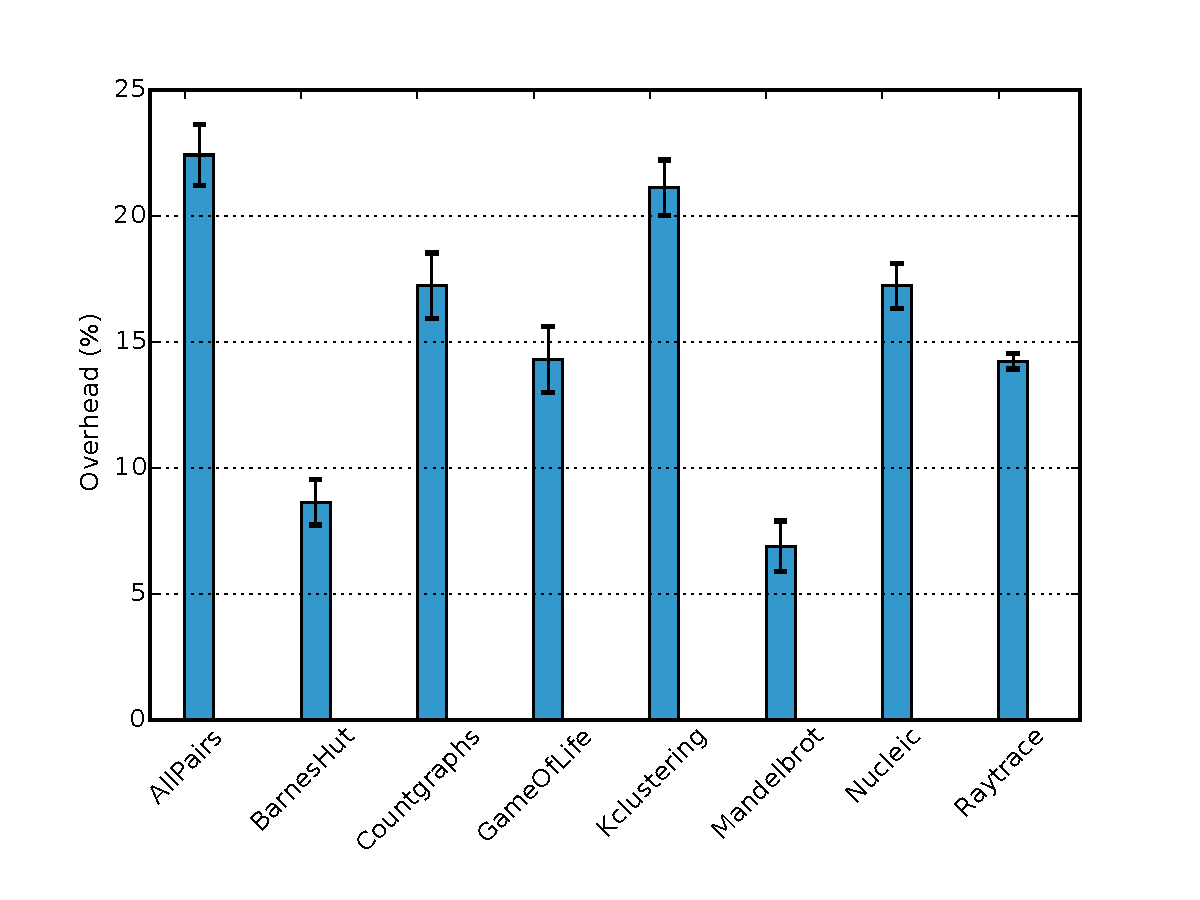
\includegraphics[width=0.9\textwidth]{Graphs/RB_overhead}
	\caption{Read barrier overhead as a percentage of mutator time.}
  \label{fig:rb-overhead}
\end{figure}

We evaluated a set of 8 benchmarks (described in Section~\ref{sec:gc_bench})
each running on all 48 cores on the SCC to measure read barrier overheads.
Figure~\ref{fig:rb-overhead} shows these overheads as a percentage of mutator
time. Our experiments reveal that, on average, the mutator spends 15.3\% of the
time executing read barriers for our benchmarks.

\begin{table}
\begin{center}
\begin{tabular} {|l|r|r|}
\hline
{\bf Benchmark} & {\bf RB invocations ($\times 10^6$)} & {\bf Forwarded}\\
\hline
{AllPairs} & 9,753 \ci{431} & 123 \ci{11} \\
{BarnesHut} & 2,864 \ci{176} & 52,702 \ci{1830} \\
{CountGraphs} & 2,584 \ci{119} & 0 \ci{0} \\
{GameOfLife} & 4,858 \ci{276} & 2,143 \ci{43}\\
{KClustering} & 3,780 \ci{265} & 101 \ci{7} \\
{Mandelbrot} & 2,980 \ci{79} & 23 \ci{3} \\
{Nucleic} & 2,887 \ci{135} & 328 \ci{21} \\
{Raytrace} & 2,217 \ci{90} & 0 \ci{0}\\
\hline
\end{tabular}
\end{center}
\caption{Effectiveness of read barrier checks: RB invocations represents the
average number of read barrier invocations and forwarded represents the average
number of instances when the read barrier encountered a forwarded object.}
\label{tab:rb_utility}
\end{table}

The next question to ask is whether the utility of the read barrier justifies
its cost. To answer this question, we measure the number of instances the read
barrier is invoked and the number of instances the barrier finds a forwarded
object (see Table~\ref{tab:rb_utility}).  We see that read barriers find
forwarded objects in less than one thousandth of a percent of the number of
instances they are invoked. Thus, in our system, the cost of read barriers is
substantial, but only rarely do they have to perform the task of forwarding
references. These results motivate our interest in a memory management design
that eliminates read barriers altogether.

\section{Procrastinating Collector (\prc)}

Eliminating read barriers, however, is non-trivial. Abstractly, one can avoid
read barriers by eagerly \emph{fixing} all references that point to forwarded
objects at the time the object is lifted to the shared heap, ensuring the
mutator will never encounter a forwarded object. Unfortunately, this requires
being able to enumerate all the references that point to the lifted object; in
general, gathering this information is very expensive as the references to an
object might originate from any object in the local heap.

We consider an alternative design that completely eliminates the need for read
barriers \emph{without} requiring a full scan of the local heap whenever an
object is lifted to the shared heap.  The design is based on the observation
that read barriers can be clearly eliminated if forwarding pointers are never
introduced.  One way to avoid introducing forwarding pointers is to
\emph{delay} operations that create them until a local garbage collection is
triggered.  In other words, rather than executing a store operation that would
trigger lifting a thread local object to the shared heap, we can simply
\emph{procrastinate}, thereby stalling the thread that needs to perform the
store.  The garbage collector must simply be informed of the need to lift the
object's closure during its next local collection. After collection is
complete, the store can take place with the source object lifted, and all
extant heap references properly adjusted.  As long as there is sufficient
concurrency to utilize existing computational resources, in the form of
available runnable threads to run other computations, the cost of
procrastination is just proportional to the cost of a context switch.

Moreover, it is not necessary to always stall an operation that involves
lifting an object to the shared heap.  We consider a new property for objects
(and their transitive object closures) called \emph{cleanliness}.  A clean
object is one that can be safely lifted to the shared heap without introducing
forwarding pointers that might be subsequently encountered by the mutator:
objects that are immutable, objects only referenced from the stack, or objects
whose set of incoming heap references is known, are obvious examples.  The
runtime analysis for cleanliness is combined with a specialized write barrier
to amortize its cost.  Thus, procrastination provides a general technique to
eliminate read barriers, while cleanliness serves as an important optimization
that avoids stalling threads unnecessarily.

The effectiveness of our approach depends on a programming model in which (a)
most objects are clean, (b) the transitive closure of the object being lifted
rarely has pointers to it from other heap allocated objects, and (c) there is a
sufficient degree of concurrency in the form of runnable threads; this avoids
idling available cores whenever a thread is stalled performing an exporting
write that involves an unclean object.  We observe that conditions (a) and (b)
are common to functional programming languages and condition (c) follows from
the \acml\ runtime model. Our technique does not rely on programmer
annotations, static analysis or compiler optimizations to eliminate read
barriers, and can be completely implemented as a lightweight runtime technique.

\subsection{Cleanliness Analysis}
\label{sec:clean}

Although \acml provides an abundance of concurrency, with the procrastination
mechanism, many of the threads in a program may end up blocked on exporting
writes, waiting for a local garbage collection to unblock them. If all of the
threads on a particular core have procrastinated, then a local garbage
collection is needed in order to make progress. Such \emph{forced} local
garbage collections make the program run longer, and hence subdue the benefit
of eliminating read barriers. Hence, it is desirable to avoid procrastination
whenever possible.

In this section, we describe our cleanliness analysis, which identifies objects
on which exporting writes do not need to be stalled. We first present auxiliary
definitions that will be utilized by cleanliness checks, and then describe the
analysis.

\subsubsection{Heap session}

Objects are allocated in the local heap by bumping the local heap frontier. In
addition, associated with each local heap is a pointer called \cf{sessionStart}
that always points to a location between the start of the heap and the
frontier. This pointer introduces the idea of a \emph{heap session}, to capture
the notion of recently allocated objects. Every local heap has exactly two
sessions: a \emph{current session} between the \cf{sessionStart} and the heap
frontier and a \emph{previous session} between the start of the heap and
\cf{sessionStart}. Heap sessions are used by the cleanliness analysis to limit
the range of heap locations that need to be scanned to test an object
closure\footnote{In the following, we write \emph{object closure} to mean the
set of objects reachable from some root on the heap; to avoid confusion, we
write \emph{function closure} to mean the representation of an SML function as
a pair of function code pointer and static environment.} for cleanliness.
Assigning the current local heap frontier to the \cf{sessionStart} pointer
starts a new session. We start a new session on a context switch, a local
garbage collection and after an object has been lifted to the shared heap.

\subsubsection{Reference count}

We introduce a limited reference counting mechanism for local heap objects that
counts the number of references from other local heap objects. Importantly, we
do not consider references from ML thread stacks. The reference count is
meaningful only for objects reachable in the current session. For such objects,
the number of references to an object can be one of four values: \cf{ZERO},
\cf{ONE}, \cf{LOCAL\_MANY}, and \cf{GLOBAL}. We steal 2 bits from the object
header to record this information. A reference count of \cf{ZERO} indicates
that the object only has references from registers or stacks, while an object
with a count of \cf{ONE} has exactly one pointer from the current session. A
count of \cf{LOCAL\_MANY} indicates that this object has more than one
reference, but that all of these references originate from the current session.
\cf{GLOBAL} indicates that the object has at least one reference that
originates from outside the current session.

\begin{figure}
\centering
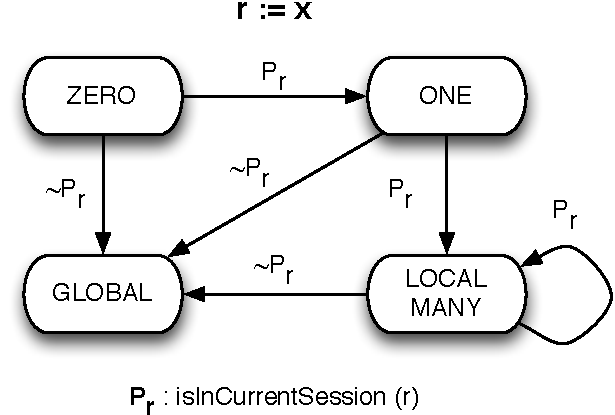
\includegraphics[width=0.6\textwidth]{Figures/std_reference_count}
\caption{State transition diagram detailing the behavior of the reference
counting mechanism with respect to object \cf{x} involved in an assignment,
\cf{r := x}, where \cf{P}$_\textrm{\cf{r}}$ = \cf{isInCurrentSession(r)}.}
\label{fig:std_ref_count}
\end{figure}

The reference counting mechanism is implemented as a part of the write barrier
(Lines 13--22 in Figure~\ref{code:writeBarrier}).
Figure~\ref{fig:std_ref_count} illustrates the state transition diagram for the
reference counting mechanism. Observe that reference counts are non-decreasing.
Hence, the reference count of any object represents the maximum number of
references that pointed to the object at any point in its lifetime.

\subsubsection{Cleanliness}

An object closure is said to be clean, if for each object reachable from the
root of the object closure,

\begin{itemize}
\item the object is immutable or in the shared heap. Or,
\item the object is the root, and has \cf{ZERO} references. Or,
\item the object is not the root, and has \cf{ONE} reference. Or,
\item the object is not the root, has \cf{LOCAL\_MANY} references, and is in the
current session.
\end{itemize}

\noindent Otherwise, the object closure is not clean.

\begin{figure}
\begin{lstlisting}
bool isClean (pointer p, bool* isLocalMany) {
  clean = true;
  foreach o in reachable(p) {
    if (!isMutable(o) || isInSharedHeap(o))
      continue;
    nv = getRefCount(o);
    if (nv == ZERO)
      clean &&= true;
    else if (nv == ONE)
      clean &&= (o != p);
    else if (nv == LOCAL_MANY) {
      clean &&= (isInCurrentSession(o));
      *isLocalMany = true;
    }
    else
      clean = false;
  }
  return clean;
}
\end{lstlisting}
\caption{Cleanliness check.}
\label{code:cleanliness}
\end{figure}

Figure~\ref{code:cleanliness} shows an implementation of an object closure
cleanliness check. Since the cleanliness check, memory barriers, and the
garbage collector are implemented in low-level code (C, assembly and low-level
intermediate language in the compiler), this code snippet, and others that
follow in this section are in pseudo-C language, to better represent their
implementation. If the source of an exporting assignment is immutable, we can
make a copy of the immutable object in the shared heap, and avoid introducing
references to forwarded objects. Standard ML does not allow the programmer to
test the referential equality of immutable objects. Equality of immutable
objects is always computed by structure. Hence, it is safe to replicate
immutable objects. If the object is already in the shared heap, there is no
need to move this object.

\begin{figure}
\centering
\subfigure[Tree-structured object closure]{\label{fig:cleanliness_tree}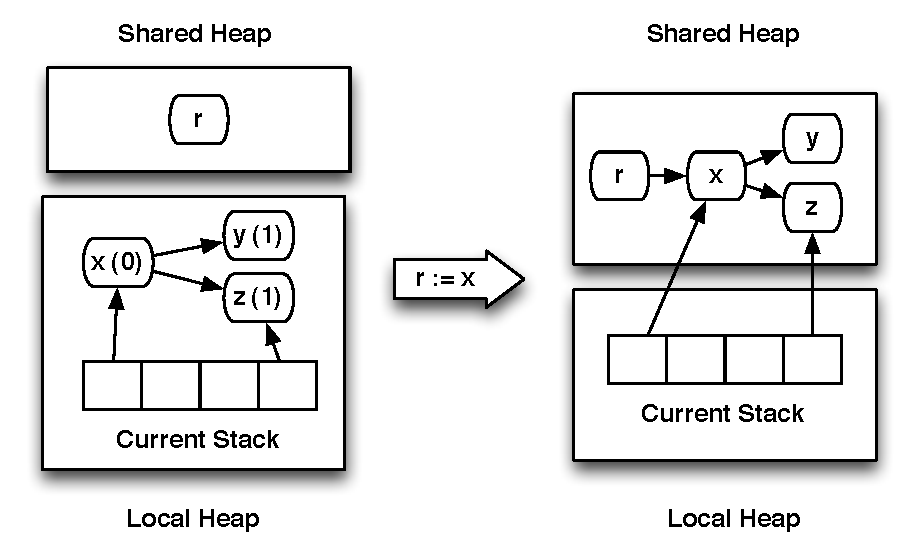
\includegraphics[width=0.8\textwidth]{Figures/Cleanliness_Tree}}\\
\subfigure[Session-based cleanliness]{\label{fig:cleanliness_session}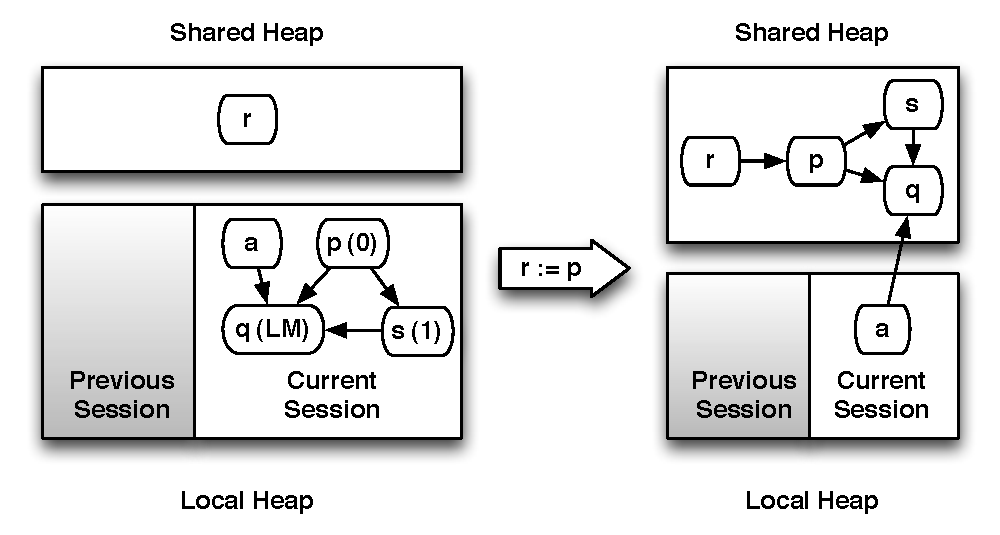
\includegraphics[width=0.8\textwidth]{Figures/Cleanliness_Session}}
\caption{Utilizing object closure cleanliness information for exporting writes to avoid references to forwarded objects.}
\label{fig:cleanliness_examples}
\end{figure}

If the object closure of the source of a exporting write is clean, we can move
the object closure to the shared heap and quickly fix all of the forwarding
pointers that might be generated. For example, consider an object that defines
a tree structure; such an object is clean if the root has \cf{ZERO} references
and all of its internal nodes have \cf{ONE} reference from their parent.  A
root having \cf{ZERO} references means it is accessed only via the stack; if it
had a count of \cf{ONE}, the outstanding reference may emanate from the heap.
Internal nodes having a reference count of \cf{ONE} implies they are reachable
only via other nodes in the object being traced.
Figure~\ref{fig:cleanliness_tree} shows such an object closure. In this
example, we assume that all objects in the object closure are mutable. The
reference count of relevant nodes is given in the brackets.  Both the root and
internal nodes can have pointers from the current stack not tracked by the
reference count. After lifting the object closure, the references originating
from the current stack are fixed by walking the stack.

Object closures need not just be trees and can be arbitrary graphs, with
multiple incoming edges to a particular object in the object closure. How do we
determine if the incoming edges to an object originate from the object closure
or from outside the object closure (from the local heap)? We cannot answer this
question without walking the local heap. Hence, we simplify the question to
asking whether all the pointers to an object originate from the current
session. This question is answered in the affirmative if an object has a
reference count of \cf{LOCAL\_MANY} (lines 11--13 in
Figure~\ref{code:cleanliness}).

Figure~\ref{fig:cleanliness_session} shows an example of a object closure whose
objects have at most \cf{LOCAL\_MANY} references. Again, we assume that all
objects in the object closure are mutable. In the transitive object closure
rooted at \cf{p}, object \cf{q} has locally many references. These references
might originate from the object closure itself (edges \cf{p $\rightarrow$ q}
and \cf{s $\rightarrow$ q}) or from outside the object closure (edge \cf{a
$\rightarrow$ q}). After lifting such object closures to the shared heap, only
the current session is walked to fix all of the references to forwarded objects
created during the copy. In practice (Section~\ref{sec:impact_session}),
current session sizes are much smaller than heap sizes, and hence exporting
writes can be performed quickly.

Finally, in the case of \cf{LOCAL\_MANY} references, the object closure is
clean, but unlike other cases, after lifting the object closure to the shared
heap, the current session must be walked to fix any references to forwarded
objects. This is indicated to the caller of \cf{isClean} function by assigning
\cf{true} to \cf{*isLocalMany}, and is used in the implementation of lifting an
object closure to the shared heap (Figure~\ref{code:lift}).

\subsection{Write barrier}
\label{sec:write_barrier}

\begin{figure}
\begin{lstlisting}
Val writeBarrier (Ref r, Val v) {
  if (isObjptr(v)) {
    //Lift if clean or procrastinate
    if (isInSharedHeap(r) &&
        isInLocalHeap(v)) {
      isLocalMany = false;
      if (isClean(v, &isLocalMany))
        v = lift(v, isLocalMany);
      else
        v = suspendTillGCAndLift(v);
    }
    //Tracking cleanliness
    if (isInLocalHeap (r) &&
        isInLocalHeap(v)) {
      n = getRefCount(v);
      if (!isInCurrentSession (r))
        setNumRefs(v, GLOBAL);
      else if (n == ZERO)
        setNumRefs(v, ONE);
      else if (n < GLOBAL)
        setNumRefs(v, LOCAL_MANY);
    }
  }
  return v;
}
\end{lstlisting}
\caption{Write barrier implementation.}
\label{code:writeBarrier}
\end{figure}

In this section, we present the modifications to the write barrier to eliminate
the possibility of creating references from reachable objects in the local heap
to a forwarded object. The implementation of our write barrier is presented in
Figure~\ref{code:writeBarrier}. A write barrier is invoked prior to a write and
returns a new value for the source of the write. The check \cf{isObjptr} at
line 2 returns true only for heap allocated objects, and is a compile time
check. Hence, for primitive valued writes, there is no write barrier. Lines 4
and 5 check whether the write is exporting. If the source of the object is
clean, we lift the transitive object closure to the shared heap and return the
new location of the object in the shared heap.

\subsubsection{Delaying writes}

If the source of an exporting write is not clean, we suspend the current thread
and switch to another thread in our scheduler. The source of the write is added
to a queue of objects that are waiting to be lifted. Since the write is not
performed, no forwarded pointers are created. If programs have ample amounts of
concurrency, there will be other threads that are waiting to be run.  However,
if all threads on a given core are blocked on a write, we move all of the
object closures that are waiting to be lifted to the shared heap. We then force
a local garbage collection, which will, as a part of the collection, fix all of
the references to point to the new (lifted) location on the shared heap. Thus,
the mutator never encounters a reference to a forwarded object. \\

\subsubsection{Lifting objects to the shared heap}

\begin{figure}
\begin{lstlisting}
Set imSet;
void liftHelper (pointer* op, pointer* frontierP) {
  frontier = *frontierP;
  o = *op;
  if (isInSharedHeap(o)) return;
  copyObject (o, frontier);
  *op = frontier + headerSize(o);
  *frontierP = frontier + objectSize(o);
  if (isMutable(o)) { setHeader(o, FORWARDED); *o = *op; }
  else imSet += o;
}

pointer lift (pointer op, bool isLocalMany) {
  start = frontier = getSharedHeapFrontier();
  imSet = {};
  //Lift transitive object closure
  liftHelper (&op, &frontier);
  foreachObjptrInRange (start, &frontier, liftHelper);
  setSharedHeapFrontier(frontier);
  //Fix forwarding pointers
  foreachObjptrInObject (getCurrentStack(), fixFwdPtr);
  foreach o in imSet { foreachObjptrInObject(o, fixFwdPtr); }
  frontier = getLocalHeapFrontier();
  if (isLocalMany)
    foreachObjptrInRange(getSessionStart(),&frontier,fixFwdPtr);
  setSessionStart(frontier);
  return op;
}
\end{lstlisting}
\caption{Lifting an object closure to the shared heap.}
\label{code:lift}
\end{figure}


Figure~\ref{code:lift} shows the pseudo-C code for lifting object closures to
the shared heap. The function \cf{lift} takes as input the root of a clean
object closure and a Boolean representing whether the object closure has any
object that has \cf{LOCAL\_MANY} references. For simplicity of presentation, we
assume that the shared heap has enough space reserved for the transitive object
closure of the object being lifted. In practice, the lifting process requests
additional shared heap chunks to be reserved for the current processor, or
triggers a shared heap collection if there is no additional space in the shared
heap.

Objects are transitively lifted to the shared heap, starting from the root, in
the obvious way (Lines 17--18). As a part of lifting, mutable objects are
lifted and a forwarding pointer is created in their original location, while
immutable objects are copied and their location added to \cf{imSet} (Lines
9--10). After lifting the transitive object closure to the shared heap, the
shared heap frontier is updated to the new location.

After object lifting, the current stack is walked to fix any references to
forwarding pointers (Line 22). Since we do not track references from the stack
for reference counting, there might be references to forwarded objects from
stacks other than the current stack. We fix such references lazily. Before a
context switch, the target stack is walked to fix any references to forwarded
objects. Since immutable objects are copied and mutable objects lifted, a
copied immutable object might point to a forwarded object. We walk all the
shared heap copies of immutable objects lifted from the local heap to fix any
references to forwarded objects (Lines 22).

Recall that if the object closure was clean, but has \cf{LOCAL\_MANY}
references, then it has at least one pointer from the current session. Hence,
in this case, we walk the current session to fix the references to any
forwarded objects to point to their shared heap counterparts (lines 24--25).
Finally, session start is moved to the current frontier.

\subsubsection{Remote spawns}
\label{sec:remote_spawns}

\begin{figure}
\begin{lstlisting}
ThreadID spawn (pointer closure, int target) {
  ThreadID tid = newThreadID();
  Thread t = newThread(closure, tid);
  isLocalMany = false;
  if (isClean(t, &isLocalMany)) {
    t = lift(t, isLocalMany);
    enqueThread(t, target);
  }
  else
    liftAndReadyBeforeGC(t, target);
  return tid;
}
\end{lstlisting}
\caption{Spawning a thread.}
\label{code:spawn}
\end{figure}

Apart from exporting writes, function closures can also escape local heaps when
threads are spawned on other cores. For spawning on other cores, the
environment of the function closure is lifted to the shared heap and then, the
function closure is added to the target core's scheduler. This might introduce
references to forwarding pointers in the spawning core's heap. We utilize the
techniques developed for exporting writes to handle remote spawns in a similar
fashion.

Figure~\ref{code:spawn} shows the implementation of thread spawn. If the
function closure is clean, we lift the function closure to the shared heap, and
enqueue the thread on the target scheduler. Otherwise, we add it to the list of
threads that need to be lifted to the shared heap. Before the next garbage
collection, these function closures are lifted to the shared heap, enqueued to
target schedulers, and the references to forwarded objects are fixed as a part
of the collection. When the target scheduler finds this new thread (as opposed
to other preempted threads), it allocates a new stack in the local heap. Hence,
except for the environment of the remotely spawned thread, all data allocated
by the thread is placed in the local heap.

\subsubsection{Barrier implementation}

In our local collector, the code for tracking cleanliness (Lines 13--24 in
Figure~\ref{code:writeBarrier}) is implemented as an RSSA pass. In RSSA, we are
able to distinguish heap allocated objects from non-heap values such as
constants, values on the stack and registers, globals, etc. This allows us to
generate barriers only when necessary.

The code for avoiding creation of references to forwarded objects (Lines 4--11
in Figure~\ref{code:writeBarrier}) is implemented in the primitive library,
where we have access to the lightweight thread scheduler.
\cf{suspendTillGCAndLift} (line 10 in Figure~\ref{code:writeBarrier}) is
carefully implemented to not contain an exporting write, which would cause
non-terminating recursive calls to the write barrier.

\section{Integrating Software-Managed Cache Coherence (\smc)}

In our next \MMSCC design, we integrate the SCC specific features into the
runtime system. Specifically, we describe a new GC design that integrates
software-managed cache coherence (SMC) capability, and utilizing the
message-passing buffers for inter-core communication. The key enabling feature
in both cases is the fact that Standard ML is a mostly functional language, and
\MM's ability to discriminate objects at runtime based on the mutability
information.

\begin{figure}
\centering
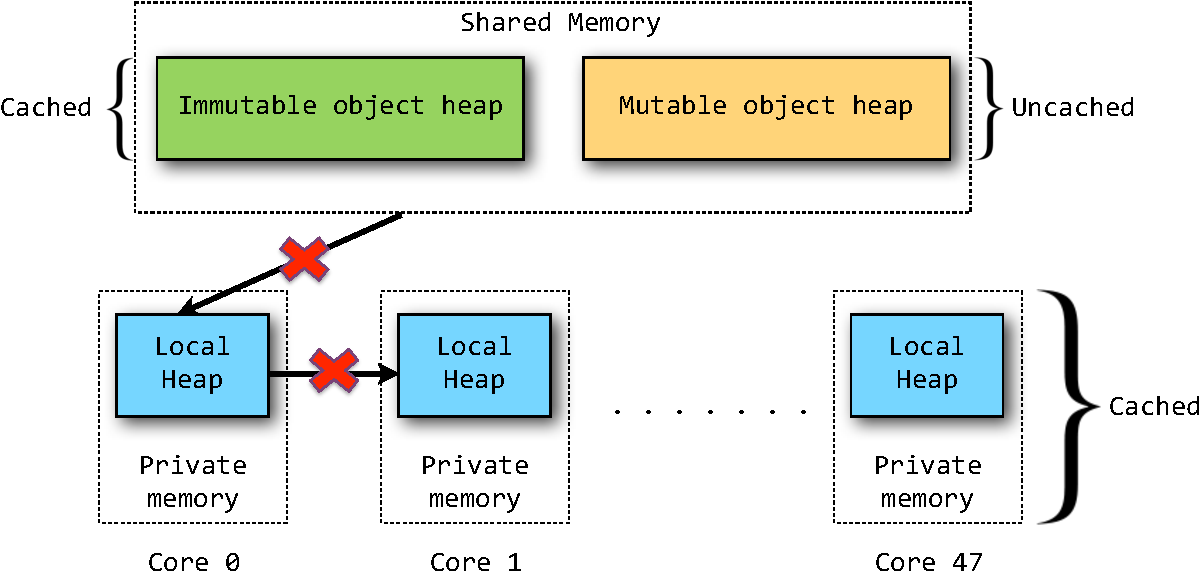
\includegraphics[width=1\textwidth]{Figures/SMC_Collector.pdf}
\caption{Heap design utilizing SCC's software-managed cache coherence capability.}
\label{fig:smc}
\end{figure}

\subsection{Heap design}

The heap design for taking advantage of SMC is given in Figure~\ref{fig:smc}.
The design is similar to the local collector design (Section~\ref{sec:lc}) with
one key difference.  Instead of a single uncached shared heap, we split our
shared heap into cached and uncached partitions. We take advantage of the fact
that standard ML can statically distinguish between mutable and immutable
objects. Since immutable objects by definition will not change after
initialization, we enable caching on one of the shared heaps into which only
globalized immutable objects will be allocated. We call this heap a cached
shared heap (CSH). Since most objects in standard ML are immutable, we gain the
advantage of caching by placing these objects in CSH while not having to deal
with coherence issues. CSH is implemented using Software Managed Coherence
(SMC) for SCC~\cite{SMC}, and we mark CSH as a MPB type area such that any
cache line from CSH will be tagged as MPB type. The CSH cached data bypasses L2
and caching operates in a write-through mode.

Caching is disabled in the uncached shared heap (USH) into which globalized
mutable objects are allocated. By disabling caching, we circumvent the
coherence issues at the cost of performance. A local heap object being
globalized might contain both mutable and immutable objects in its transitive
object closure. Hence, globalization might involve allocating new objects in
both partitions of the shared heap. For the same reason, pointers are allowed
between the two partitions of the shared heap.

\subsection{Memory Consistency}

The key challenge now is to ensure that the updates to CSH are visible to all
the cores. Since CSH is cached, and SCC does not provide hardware cache
coherence, explicit cache invalidations and flushes must be implemented.
Moreover, any missed flushes or invalidations will lead to incoherent caches,
while frequent flushes or invalidations leads to poor performance. The key
observation is that the baseline local collector design has both read and write
barriers; our idea is to integrate the cache control primitives into the memory
barriers.

\begin{figure}
\begin{lstlisting}
pointer readBarrier (pointer p) {
  if (!isPointer(p)) return p;
  if (getHeader(p) == FORWARDED) {
		/* Address in shared heap */
    p = *(pointer*)p;
		if (p > MAX_CSH_ADDR) {
			/* Address in cached shared heap, and has not
			 * been seen so far. Fetch the updates. */
			smcAcquire();
			MAX_CSH_ADDR = p;
		}
	}
  return p;
}
\end{lstlisting}
\caption{Read barrier with software-managed cache coherence capability.}
\label{code:read_barrier_smc}
\end{figure}

\begin{figure}
\begin{lstlisting}
val writeBarrier (Ref r, Val v) {
  if (isObjptr(v) &&
			isInSharedHeap(r) &&
			isInLocalHeap(v)) {
			/* Move transitive object closure to shared
			 * heap, and install forwarding pointers */
			v = globalize (v);
			/* Publish the updates */
			smcRelease();
	}
	return v;
}
\end{lstlisting}
\caption{Write barrier with software-managed cache coherence capability.}
\label{code:write_barrier_smc}
\end{figure}


The CSH is always mapped to an address that is greater than the starting
address of the USH. Each core maintains the largest address seen in CSH in the
\cf{MAX\_CSH\_ADDR} variable. During an object read, if the address of the
object lies in the shared heap and is greater than \cf{MAX\_CSH\_ADDR}, we
invalidate any cache lines that might be associated with CSH by invoking
\texttt{smcAcquire()} (Line 9 in Figure~\ref{code:read_barrier_smc}). This
ensures that the values read are not stale. We update the \cf{MAX\_CSH\_ADDR}
if necessary. Since the objects in CSH are immutable, there is no need to
perform cache invalidation while reading an address that is less than
\cf{MAX\_CSH\_ADDR}. Additionally, after garbage collection,
\cf{MAX\_CSH\_ADDR} is set to point to the start of the CSH.

Similarly, whenever an object is globalized to the CSH, we must ensure that the
updates are visible to all of the cores. After an exporting write, we invoke
\texttt{smcRelease()}, to flush any outstanding writes to the memory (Line 9 in
Figure~\ref{code:write_barrier_smc}).

\subsection{Mapping channel communication over message-passing buffers}
\label{sec:comm_opt}

In this section, we describe how we map the \MM communication model on top of
the MPB. The main challenge here is the compatibility between the \MM
communication model and the capabilities of MPB. In \MM, threads communicate
over first-class channels, which support many-to-many communication pattern.
Hence, a receiver does not know the identity of the sender and vice versa.
Moreover, if a receiver is not available, the sender thread blocks; it is
descheduled, and some other thread from the scheduler queue continues execution
on that core. Moreover, the values sent over the channels in \MM can be
mutable. The channel itself is simply a data structure implemented over shared
memory. However, the communication on the SCC over libraries such as RCCE and
RCKMPI is optimized for SPMD programming model, where the sender and the
receiver know each other's identities, and are expected to arrive at the
communicaiton point at the same time. Hence, considering the fact that MPB
memory is on 8KB, both RCCE and RCKMPI use busy waiting strategy for intercore
communication. Thus, careful design is needed to map \MM communication
abstraction over the MPB.

Our channel mapping implementation exploits both the cached shared heap and MPB
for efficient inter-core message passing. We take advantage of our heap layout
and the availability of static type information to take advantage of the fast,
on-die MPB memory. We consider the following five cases:

\begin{enumerate}
\item Channel is located in the local heap
\item Channel is located in the shared heap, and the message being sent is an
unboxed value
\item Channel is located in the shared heap, the message is in the local heap,
and at least one of the objects in the transitive closure of the message being
sent is mutable
\item Channel is located in the shared heap, the message is in the local heap,
and all objects in the transitive closure of the message being sent are
immutable
\item Channel and the message are located in the shared heap
\end{enumerate}

For case 1, we observe that only channels that are located in the shared heap
can be used for inter-core communication. Our heap invariants prevent pointers
from one local heap to another. Thus, if a channel is located in the local
heap, then no thread on the other cores have a reference to this channel. Thus,
communication under case 1 only involves a value or a pointer exchange between
the communicating lightweight threads.

MultiMLton supports unboxed types that represent raw values. Hence, under case
2, we add a reference to the thread along with the value being sent to the
channel. In addition, we add a reference to the blocked thread to the
remembered list so that the local garbage collection can trace it.

\begin{figure}
\centering
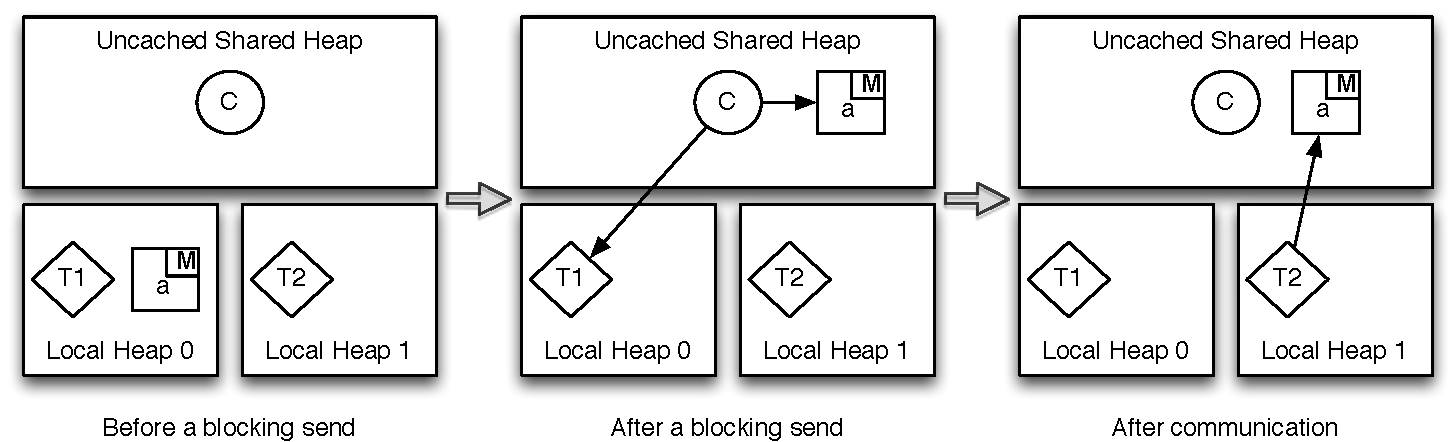
\includegraphics[width=1\textwidth]{Figures/Comm_Case_3}
\caption{Steps involved in sending an mutable object \cf{a} by thread \cf{T1}
on a shared heap channel \cf{C}, which is eventually received by thread
\cf{T2}.}
\label{fig:comm_mutable}
\end{figure}

If the message being sent has a mutable object in the transitive closure, we
must make this object visible to both the sender and the receiver core.
Figure~\ref{fig:comm_mutable} shows the case where a thread \cf{T1} sends a
mutable object \cf{a} on a shared heap channel \cf{C}. In this case, we eagerly
globalize \cf{a} before \cf{T1} blocks. Since the message is already in the
shared heap, when the receiver thread \cf{T2} eventually arrives, it just picks
up a pointer to the message in the shared heap.

\begin{figure}
\centering
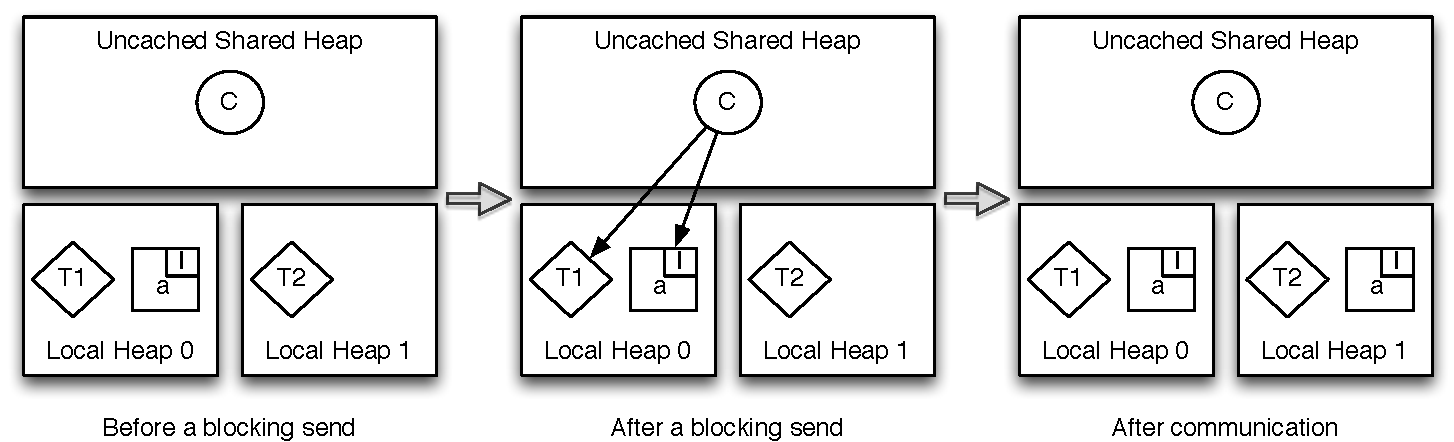
\includegraphics[width=1\textwidth]{Figures/Comm_Case_4}
\caption{Steps involved in sending an immutable object \cf{a} by thread \cf{T1}
on a shared heap channel \cf{C}, which is eventually received by thread
\cf{T2}.}
\label{fig:comm_immutable}
\end{figure}

Figure~\ref{fig:comm_immutable} shows the case where a thread \cf{T1} sends an
immutable object \cf{a} on a shared channel \cf{C}. Here, we simply add to the
channel \cf{C}, a reference to the message \cf{a} in the local heap, along with
the reference to the thread \cf{T1}. In addition, a reference to the object
\cf{a} is added to the remembered list, so that a local garbage collection will
be able to identify \cf{a} as being alive.

Afterward, when the receiver thread \cf{T2} arrives and finds the message not to
be in the shared heap, it sends an inter-core interrupt to the core on which the
message is located (core 0, in this case). After this message transfer is
initiated over the MPB using RCCE to transfer the object \cf{a} from core 0 to
core 1. Since Standard ML immutable objects do not have identity, making a copy
of the immutable object is safe under MultiMLton.

If the channel and the message are located in the shared heap, communication
only involves a value or a pointer exchange. This case is similar to case 1.

\section{Evaluation}
\label{sec:gc_bench}

The core, mesh controller, and memory on the SCC can be configured to run at
different frequencies. For our experiments we chose 533 MHz, 800 MHz, and 800
MHz for core, mesh, and memory respectively. In our results, wherever
appropriate, we present the 95\% confidence intervals, obtained using Student's
t-distribution.

For our experimental evaluation, we picked 8 benchmarks from the MLton
benchmark suite. The benchmarks were derived from sequential standard ML
implementation and were parallelized using ACML~\cite{Ziarek11}. The benchmarks
are:

\begin{itemize}
\item {\bf AllPairs}: an implementation of Floyd-Warshall algorithm for
computing all pairs shortest path.
\item {\bf BarnesHut}: an n-body simulation using Barnes-Hut algorithm.
\item {\bf CountGraphs}: computes all symmetries (automorphisms) within a set
of graphs.
\item {\bf GameOfLife}: Conway's Game of Life simulator
\item {\bf Kclustering}: a k-means clustering algorithm, where each stage is
spawned as a server.
\item {\bf Mandelbrot}: a Mandelbrot set generator.
\item {\bf Nucleic}: Pseudoknot~\cite{Pseudoknot} benchmark applied on multiple
inputs.
\item {\bf Raytrace}: a ray-tracing algorithm to render a scene.
\end{itemize}

\begin{table}
\begin{center}
\begin{tabular} {|l|r|r|r|r|}
\hline
\multirow{2}{*}{{\bf Benchmark}} & {\bf Allocation Rate} 	& \multicolumn{2}{|c|}{{\bf Allocation}} & \multirow{2}{*}{\bf \# Threads} \\
\cline{3-4}
																 & \multicolumn{1}{|c|}{{\bf (MB/s)}}						& {\bf Total (GB)} & {\bf \% Sh}	&	\\
\hline
{AllPairs} 		& 53 	\ci{2.3} & 16 \ci{0.23} 	& 11 	\ci{0.09} & 512 \\
{BarnesHut} 	& 70 	\ci{2.3} & 20 \ci{0.25} 	& 2		\ci{0.02} & 1024 \\
{CountGraphs} & 144 \ci{3.8} & 24 \ci{0.32} 	& 1		\ci{0.01} & 256 \\
{GameOfLife} 	& 127 \ci{5.0} & 21 \ci{0.47} 	& 13	\ci{0.17} & 1024 \\
{KClustering} & 108 \ci{2.9} & 32	\ci{0.31} 	& 3		\ci{0.05} & 1024 \\
{Mandelbrot} 	& 43 	\ci{1.7} & 2	\ci{0.02} 	& 8		\ci{0.03} & 512 \\
{Nucleic} 		& 87 	\ci{3.4} & 14	\ci{0.17} 	& 1		\ci{0.00} & 384 \\
{Raytrace} 		& 54 	\ci{2.6} & 12	\ci{0.14} 	& 4		\ci{0.03} & 256 \\
\hline
\end{tabular}
\end{center}
\caption{Benchmark characteristics. \%Sh represents the average fraction of
bytes allocated in the shared heap.}
\label{tab:bench_char}
\end{table}

The benchmark characteristics is given in Figure~\ref{tab:bench_char}. The
numbers were obtained using local collector (\lc) with programs running on 48
cores, and the average of the results is reported. The benchmarks were designed
such that the input size and the number of threads are tunable. Out of the
total bytes allocated during the program execution, on average 5.4\% is
allocated in the shared heap. Thus, most of the objects allocated are collected
locally, without the need for stalling all of the mutators. The allocation rate
on the SCC is typically much lower than comparable general purpose commerical
offerings. On the SCC, not only is the processor slow (533MHz) but also the
serial memory bandwidth for our experimental setup is only around 70 MB/s.

\subsection{Performance}

\begin{figure}
  \centering
  \subfigure[Speedup]{\label{fig:speedup}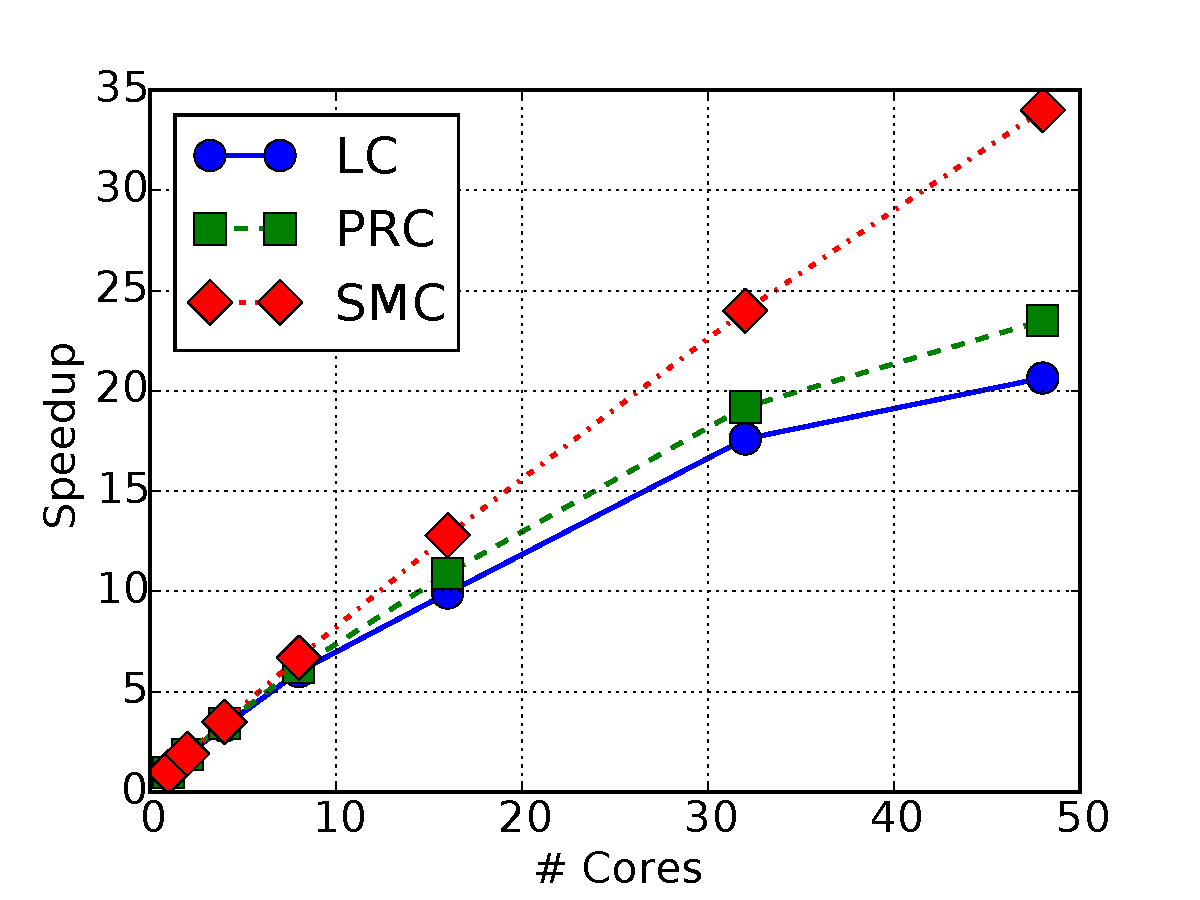
\includegraphics[width=0.45\textwidth]{Graphs/speedup_scc_heap}}
  \subfigure[Total time (48 cores)]{\label{fig:time_SCC}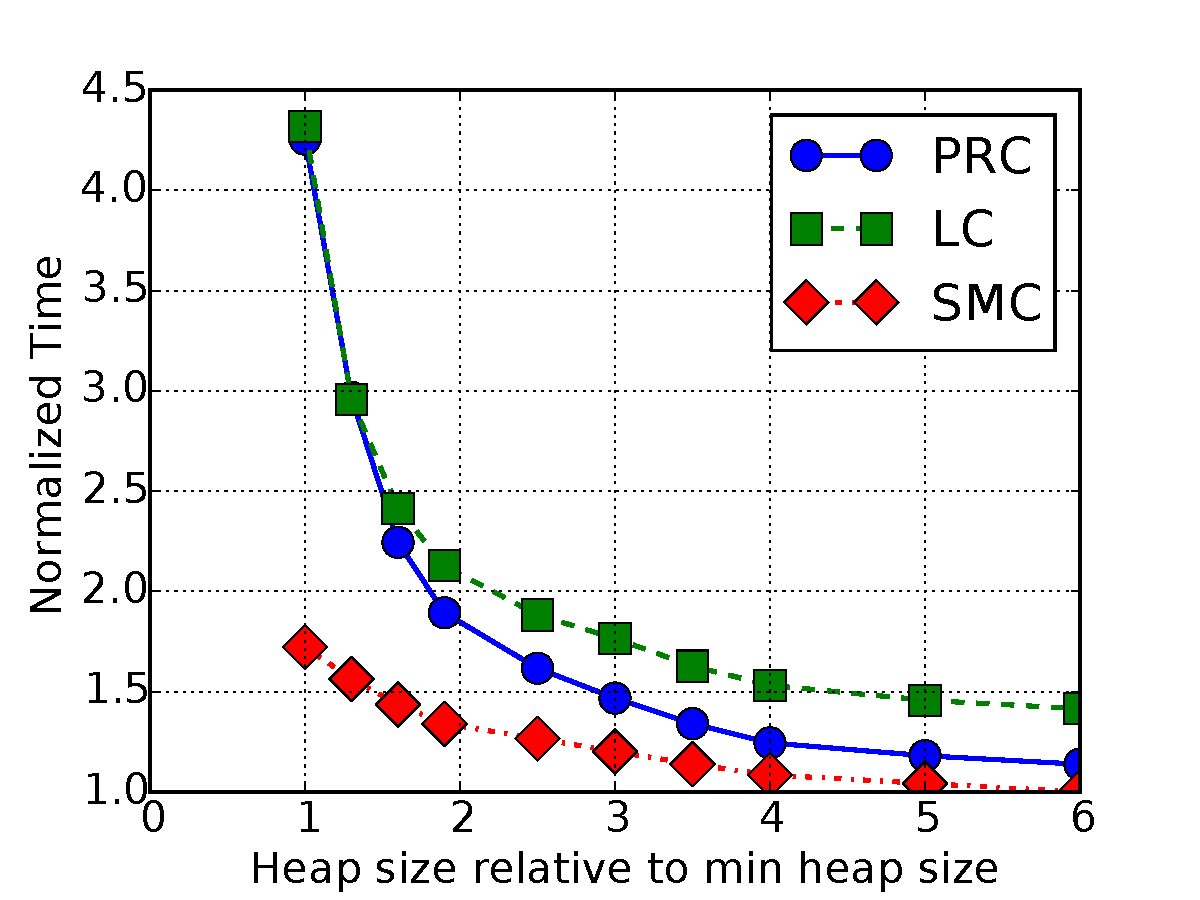
\includegraphics[width=0.45\textwidth]{Graphs/time_scc}}
  \subfigure[Mutator time (48 cores)]{\label{fig:mutator_time_SCC}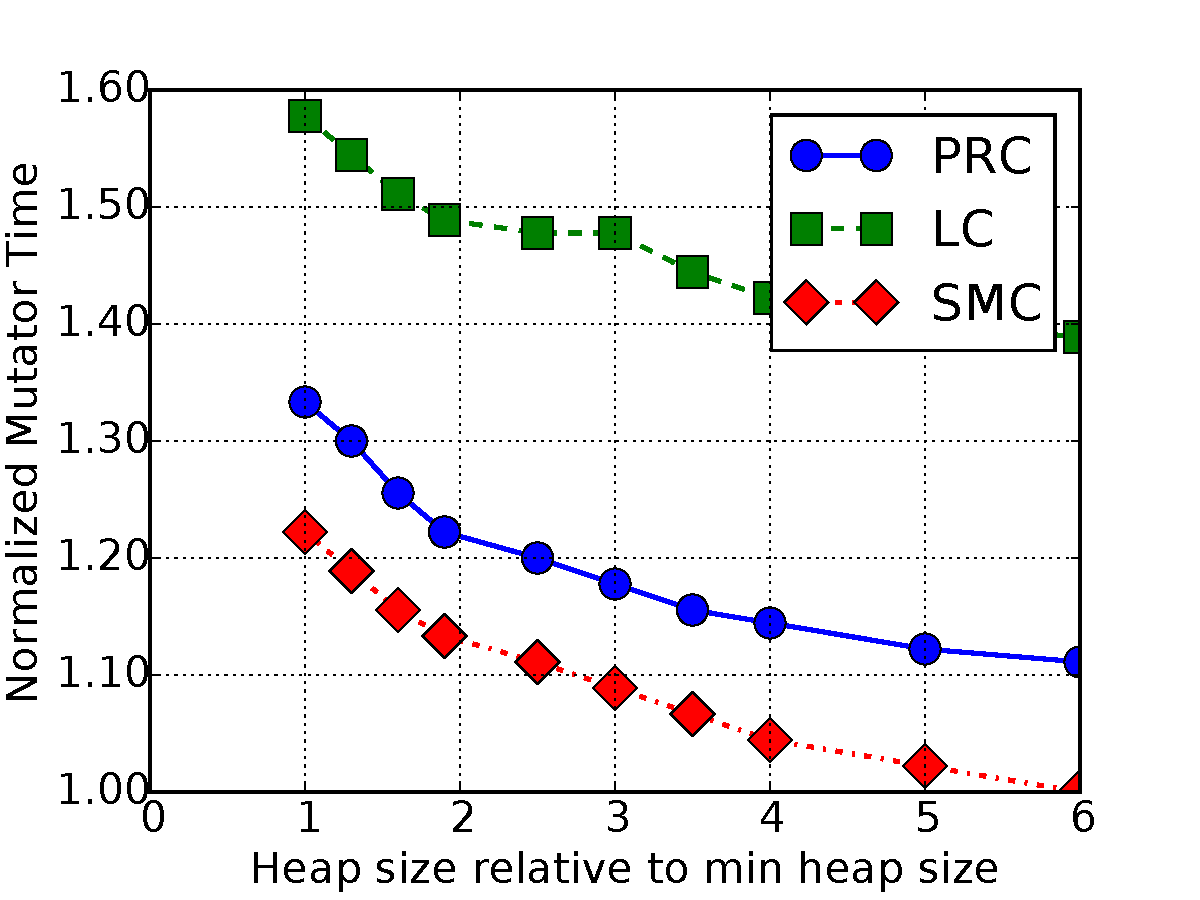
\includegraphics[width=0.45\textwidth]{Graphs/mutator_time_scc}}
  \subfigure[GC time (48 cores)]{\label{fig:gc_time_SCC}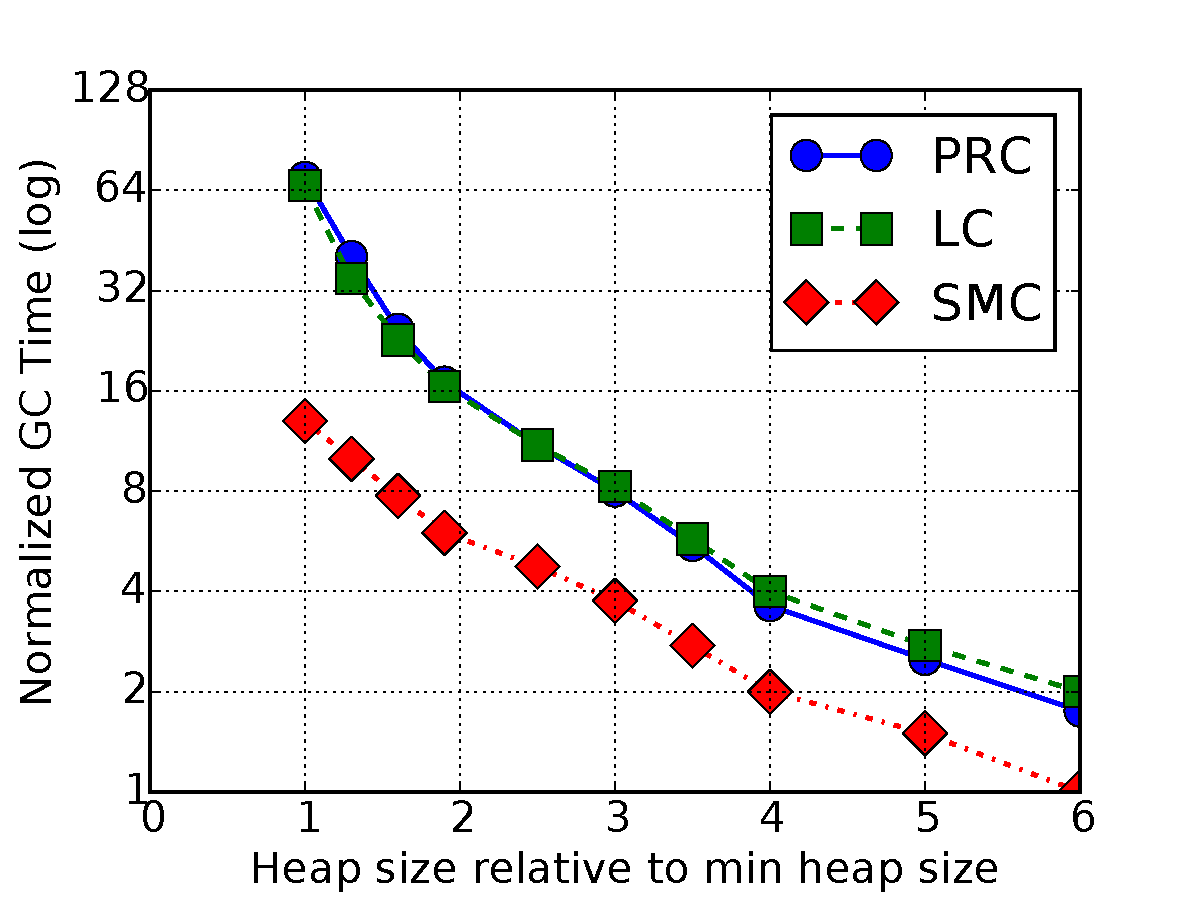
\includegraphics[width=0.45\textwidth]{Graphs/gc_time_scc}}
	\caption{Performance comparison of local collector with read barriers (\lc),
	procrastinating collector without read barriers (\prc), and collector
	utilizing software-managed cache coherence (SMC) : Geometric mean for 8
	benchmarks.}
  \label{fig:time}
\end{figure}

Figurue~\ref{fig:time} presents the speedup results and illustrates space-time
trade-offs critical for any garbage collector evaluation. Among the three
variants, SMC performs the best (Figure~\ref{fig:speedup}) due to the fact that
most of the accesses under SMC is cached, unlike \lc and \prc. We also see that
the performance of \lc and \prc start to flatten out due to the contention on the
uncached shared memory as we increase the number of cores. Thus, with
increasing number of cores, the uncached shared memory becomes the bottleneck.

As we decrease the overall heap size, we see that the programs take longer to
run, due to the more frequent GCs (Figure~\ref{fig:time_SCC}). The reduction in
heap size, by definition, does not adversely affect the mutator time when
compared with the GC time. At 3$\times$ the minimum heap size under which the
programs would run, \prc is 17\% faster than \lc, and SMC is 18\% faster than
\prc. Overall, SMC is 32\% faster than \lc.

The mutator time (Figure~\ref{fig:mutator_time_SCC}) of \lc is consistently
higher than \prc due to the elimination of read barrier overheads under \prc.
Although SMC does have read barrier overheads, caching much of the shared
memory accesses keeps the mutator time low. We instrumented our read and write
barriers to classify the memory accesses. On average, across all of the
benchmarks, 89\% of the read or write requests were to the local heap, which is
private and is cached both in L1 and L2. This is common to all three versions
of the local collector. Thus, SMC derives mutator gains by caching much of the
11\% of the GC requests.

Out of the shared heap memory requests, on average, 93\% of all requests were
to the cached shared heap. However, it should be noted that cached shared heap
data bypass L2, and are only cached in the comparatively smaller L1 cache.
Hence, the benefit of caching shared heap data, as far as the mutator is
concerned, may not be dramatic if the cached shared heap reads are far and few
between. In any case, with SMC, less than 1\% of mutator accesses were to the
uncached memory. Thus, SMC is able to potentially cache more than 99\% of
memory accesses.

There is very little difference between the GC times
(Figure~\ref{fig:gc_time_SCC}) between \lc and \prc. This is because both the
variants are similar in terms of the actual GC work. However, SMC's GC time
tends to be lower since part of the expensive shared heap collection itself is
cached. Thus, software-managed cache coherence not only benefits the mutator
but also the garbage collector.

\subsection{Evaluating Procrastinating Collector}

In this section, we will focus on the procrastinating collector (\prc) design,
and analyze the impact of different optimizations.

\subsubsection{Impact of cleanliness}
\label{sec:impact_cleanliness}

Cleanliness information allows the runtime system to avoid preempting threads
on a write barrier when the source of an exporting write is clean. In order to
study the impact of cleanliness, we removed the reference counting code and
cleanliness check from the write barrier; thus, every exporting write results
in a thread preemption and stall. The results presented here were taken with
programs running on 48-cores.

\begin{table}
\begin{center}
\begin{tabular} {|l|r|r|r|}
\hline
{\bf Benchmark} & {\bf \prc} & {\bf \prc MU-} & {\bf \prc CL-} \\
\hline
AllPairs 		& 604 \ci{42}		&	616 \ci{43}			&	28573 \ci{1429} \\
BarnesHut 	& 8376 \ci{503}	&	82284 \ci{3291}	& 23504887 \ci{1175244} \\
CountGraphs & 45 \ci{2}			&	64 \ci{2}				& 17061 \ci{1194} \\
GameOfLife 	& 11973 \ci{359} &	238462 \ci{16692}	& 1936250 \ci{58088} \\
KClustering & 7227 \ci{217}	& 15394 \ci{616}	& 8107173 \ci{405359} \\
Mandelbrot 	& 44 \ci{2}			& 84 \ci{5}				& 5863 \ci{235} \\
Nucleic 		& 58 \ci{3}			& 104594 \ci{4184}	&	209840 \ci{14689} \\
Raytrace 		& 881 \ci{35}		& 973 \ci{39}			& 13464 \ci{404} \\
\hline
\end{tabular}
\end{center}
\caption{Average number of preemptions on write barrier.}
\label{tab:preempt}
\end{table}

Table~\ref{tab:preempt} shows the number of preemptions on write barrier for
different configurations. \prc represents the variant with all of the features
enabled; \prc MU- shows a cleanliness optimization that does not take an
object's mutability into consideration in determining cleanliness (using only
recorded reference counts instead), and \prc CL- represents preemptions incurred
when the collector does not use any cleanliness information at all. Without
cleanliness, on average, the programs perform substantially more preemptions
when encountering a write barrier.

Recall that if all of the threads belonging to a core get preempted on a write
barrier, a local major GC is \emph{forced}, which lifts all of the sources of
exporting writes, fixes the references to forwarding pointers and unblocks the
stalled threads. Hence, an increase in the number of preemptions leads to an
increase in the number of local collections.

\begin{table}
\begin{center}
\begin{tabular} {|l|r|r|r|}
\hline
{\bf Benchmark} & {\bf \prc} & {\bf \prc MU-} & {\bf \prc CL-} \\
\hline
AllPairs & 0.08 \ci{0} & 0.08 \ci{0} & 38.55 \ci{2.31} \\
BarnesHut & 0.17 \ci{0.01} & 19.2 \ci{0.96} & 100 \ci{3} \\
CountGraphs & 0 \ci{0} & 0.03 \ci{0} & 0.18 \ci{0.01} \\
GameOfLife & 3.54 \ci{0.21} & 9.47 \ci{0.47} & 99.75 \ci{4.99} \\
KClustering & 0 \ci{0} & 0.02 \ci{0} & 21.64 \ci{1.08} \\
Mandelbrot & 1.43 \ci{0.1} & 2.86 \ci{0.11} & 86.22 \ci{6.04} \\
Nucleic & 0 \ci{0} & 9.37 \ci{0.28} & 19.3 \ci{0.58} \\
Raytrace & 1.72 \ci{0.1} & 1.72 \ci{0.07} & 24.86 \ci{0.99} \\
\hline
\end{tabular}
\end{center}
\caption{Average percentage of forced GCs out of the total number of local
major GCs.}
\label{tab:forcedGCs}
\end{table}

Table~\ref{tab:forcedGCs} shows the percentage of local major GCs that were
forced compared to the total number of local major GCs. \prc CL- shows the
percentage of forced GCs if cleanliness information is not used. On average,
49\% of local major collection performed is due to forced GCs if cleanliness
information is not used, whereas it is less than 1\% otherwise.  On benchmarks
like {\tt BarnesHut}, {\tt GameOfLife} and {\tt Mandelbrot}, where all of the
threads tend to operate on a shared global data structure, there are a large
number of exporting writes. On such benchmarks almost all local GCs are forced
in the absence of cleanliness. This adversely affects the running time of
programs.

\begin{figure}
  \centering
  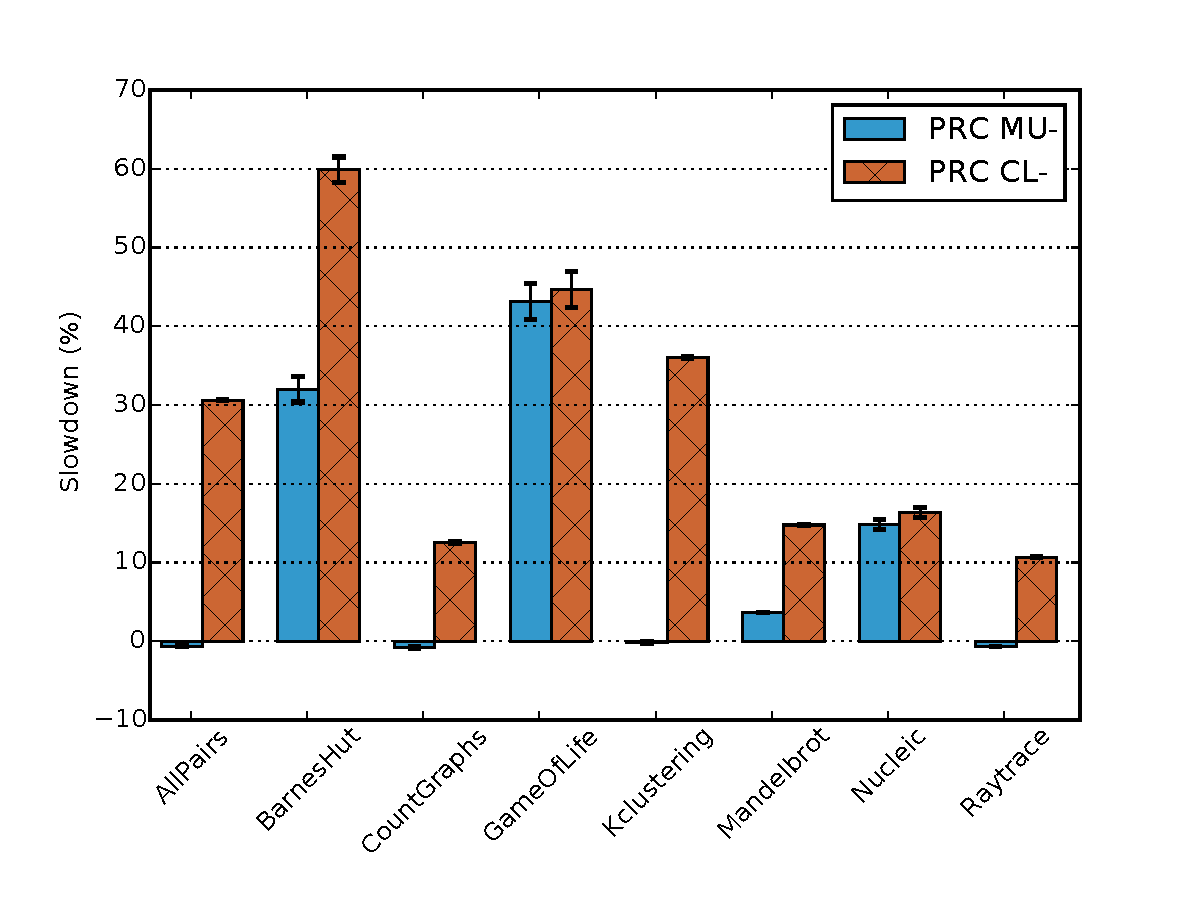
\includegraphics[width=\textwidth]{Graphs/slowdown_cleanliness}
	\caption{Impact of utilizing object mutability information and cleanliness
	analysis on the performance of \prc.}
  \label{fig:slowdown-cleanliness}
\end{figure}

Figure~\ref{fig:slowdown-cleanliness} shows the running time of programs
without using cleanliness. On average, programs tend to run 28.2\% slower if
cleanliness information is ignored. The results show that cleanliness analysis
therefore plays a significant role in the \prc design.

\subsubsection{Impact of immutability}

If the source of an exporting write is immutable, we can make a copy of the
object in the shared heap and assign a reference to the new shared heap object
to the target. Hence, we can ignore the reference count of such objects. Not
all languages may have the ability to distinguish between mutable and immutable
objects in the compiler or in the runtime system. Hence, we study the impact of
our local collector design with mutability information in mind.  To do this, we
ignore the test for mutability in the cleanliness check
(Figure~\ref{code:cleanliness}) and modify the object lifting code in
Figure~\ref{code:lift} to treat all objects as mutable.

\prc MU- in Table~\ref{tab:preempt} and Table~\ref{tab:forcedGCs} show the
number of write barrier preemptions and the percentage of forced GCs,
respectively, if all objects were treated as mutable.  For some programs such
as {\tt AllPairs}, {\tt CountGraphs}, or {\tt Kclustering}, object mutability
does not play a significant factor.  For benchmarks where it does,
distinguishing between mutable and immutable objects helps avoid inducing
preemptions on a write barrier since a copy of the immutable object can be
created in the shared heap without the need to repair existing references to
the local heap copy.

Figure~\ref{fig:slowdown-cleanliness} shows the performance impact of taking
object mutability into account. While ignoring object mutability information,
{\tt BarnesHut}, {\tt GameOfLife} and {\tt Nucleic} are slower due to the
increased number of forced GCs. Interestingly, {\tt AllPairs}, {\tt
CountGraphs}, {\tt Kclu\allowbreak stering} and {\tt Raytrace} are marginally
faster if the mutability information is ignored. This is due to not having to
manipulate the \cf{imSet} (Line 15 in Figure~\ref{code:lift}), and walking
immutable objects after the objects are lifted (Line 22 in
Figure~\ref{code:lift}). On average, we see a 11.4\% performance loss if
mutability information is not utilized for cleanliness.

\subsubsection{Impact of heap session}
\label{sec:impact_session}

\begin{table}
\begin{center}
\begin{tabular} {|l|r|r|r|}
\hline
{\bf Benchmark} & {\bf \% LM Clean} & {\bf Avg. Session Size (Bytes)} \\
\hline
AllPairs & 5.35 \ci{0.37} & 2966 \ci{119} \\
Barneshut & 13.27 \ci{0.53} & 1596 \ci{96} \\
Countgraphs & 8.86 \ci{0.53} & 3648 \ci{73} \\
GameOfLife & 23.9 \ci{1.2} & 1384 \ci{55} \\
Kclustering & 18.13 \ci{0.54} & 2248 \ci{135} \\
Mandelbrot & 4.64 \ci{0.09} & 8549 \ci{598} \\
Nucleic & 13.3 \ci{0.27} & 1226 \ci{37} \\
Raytrace & 8.28 \ci{0.41} & 1112 \ci{22} \\
\hline
\end{tabular}
\end{center}
\caption{Impact of heap session: \% LM clean represents the fraction of
instances when a clean object closure has at least one object with
\cf{LOCAL\_MANY} references.}
\label{tab:session-impact}
\end{table}

In order to assess the effectiveness of using heap sessions, we measured the
percentage of instances where the source of an exporting write is clean with at
least one of the objects in the closure has a \cf{LOCAL\_MANY} reference.
During such instances, we walk the current heap session to fix any references
to forwarded objects. Without using heap sessions, we would have preempted the
thread in the write barrier, reducing  available concurrency. The results are
presented in Table~\ref{tab:session-impact}.

The first column shows the percentage of instances when an object closure is
clean and has at least one object with \cf{LOCAL\_MANY} references. On average,
we see that 12\% of clean closures have at least one object with
\cf{LOCAL\_MANY} references. We also measured the average size of heap sessions
when the session is traced as a part of lifting an object closure to the shared
heap (Line 25 in Figure~\ref{code:lift}). The average size of a heap session
when it is traced is 2859 bytes, which is less than a page size. These results
show that utilizing heap sessions significantly contributes to objects being
tagged as clean, and heap sessions are small enough to not introduce
significant overheads during tracing.


\subsection{MPB mapped channels}

\begin{figure}[ht]
\centering
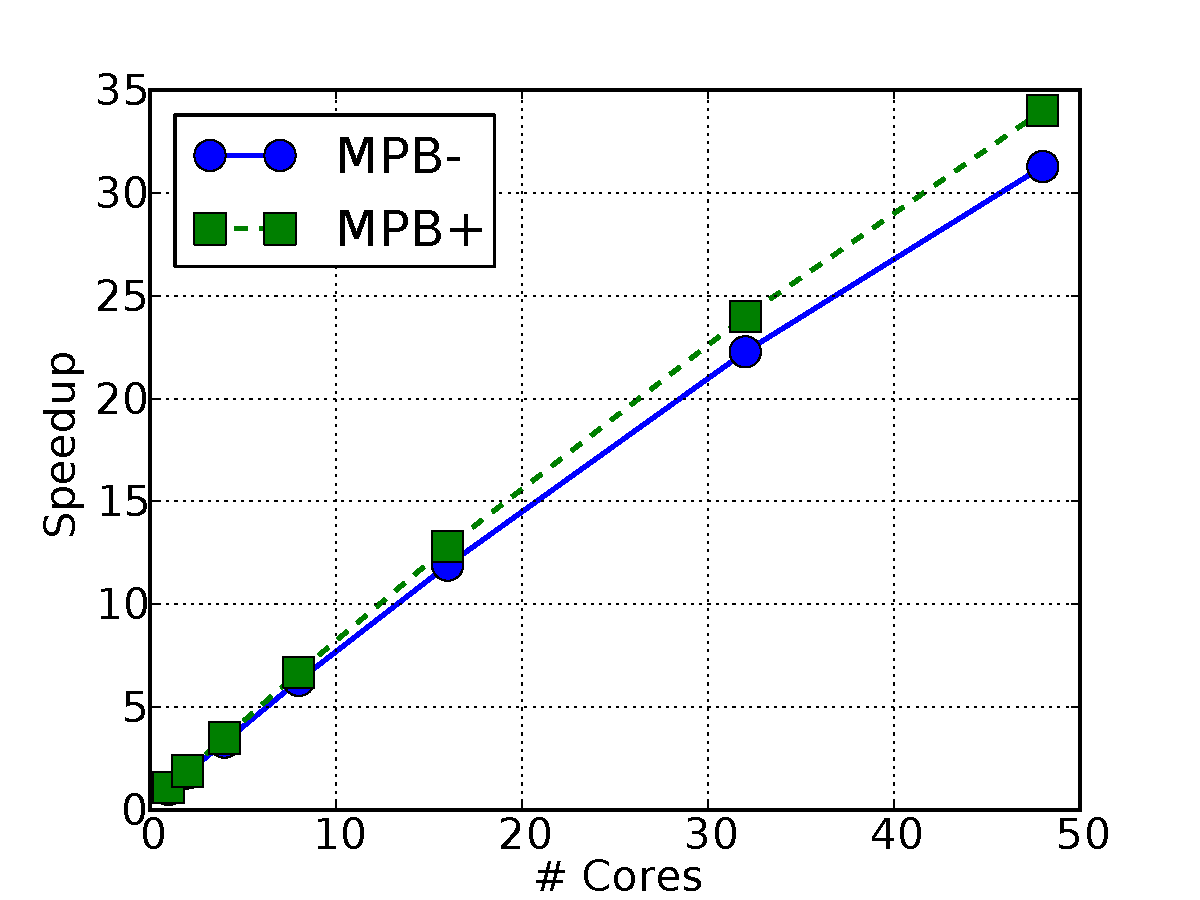
\includegraphics[width=1\textwidth]{Graphs/speedup_scc_chan}
\caption{Performance comparison of first-class channel communication over the
MPB \cf{(MBP+)} vs solely over the shared memory \cf{(MPB-)}: Geometric mean
over 8 benchmarks.}
\label{fig:speedup_scc_chan}
\end{figure}


In this section, we study the impact of MPB mapped channels. In order to
evaluate the benefit of mapping the first-class channel communication over the
message passing buffer memory, we implemented a version of our communication
library that does not use the message passing buffer memory. Recall that if the
channel is located in the shared heap, the message in the local heap, and the
message does not have a mutable object in its transitive closure, we perform
the transfer over the message passing buffer (Case 4 in
Section~\ref{sec:comm_opt}). Instead, we eagerly globalize the transitive
closure of the message and just share the pointer with the receiving thread
(similar to Case 3). We call this version MPB-, and the original version MPB+.

Figure~\ref{fig:speedup_scc_chan} shows the performance comparison of MPB+
versus MPB-. On 48-cores, MPB+ is only around 9\% faster than the MPB- version.
We can attribute several reasons for this marginal improvement. First, we
observed that, on average, around only 32\% of channel communications were
taking advantage of the MPB (Case 4) in the case of MPB+. The rest of the
channel communications were either local or were using the shared memory to
transfer the messages. Moreover, in the case of MPB-, immutable inter-core
messages are transferred over the CSH which is cached.

Second, the cost of inter-core interrupts is substantial, as was observed by
others~\cite{Peter11,Darko11}. We measured the time it takes between a core
issuing an inter-core interrupt to the time it sends or receives the first byte
is around 2000 core cycles. Since majority of the immutable messages exchanged
between cores are small, the overhead of setting up the message transfer
outweighs the benefit of using the MPB. However, utilizing the MPB prevents
immutable messages from being globalized, thus reducing the pressure on the
shared memory. As a result, the number of expensive shared heap collections are
reduced.

\section{Related Work}

Over the years, several local collector designs ~\cite{Steele75, Doligez93,
Steensgaard00, Anderson10} have been proposed for multithreaded programs.
Recently, variations of local collector design have been adopted for
multithreaded, functional language runtimes like GHC~\cite{Marlow11} and
Manticore~\cite{Auhagen11}. Doligez et al.~\cite{Doligez93} proposed a local
collector design for ML with threads where all mutable objects are allocated
directly on the shared heap, and immutable objects are allocated in the local
heap. Similar to our technique, whenever local objects are shared between
cores, a copy of the immutable object is made in the shared heap. Although this
design avoids the need for read and write barriers, allocating all mutable
objects, irrespective of their sharing characteristics can lead to poor
performance due to increased number of shared collections, and memory access
overhead due to NUMA effects and uncached shared memory as in the case of SCC.
It is for this reason we do not treat the shared memory as the oldest
generation for our local generation collector unlike other
designs~\cite{Doligez93, Marlow11}.

Several designs utilize static analysis to determine objects that might
potentially escape to other threads~\cite{Jones05, Steensgaard00}. Objects that
do not escape are allocated locally, while all others are allocated in the
shared heap. The usefulness of such techniques depends greatly on the precision
of the analysis, as objects that might potentially be shared are allocated on
the shared heap. This is undesirable for architectures like the SCC where
shared memory accesses are very expensive compared to local accesses. Compared
to these techniques, our design only exports objects that are definitely shared
between two or more cores. Our technique is also agnostic to the source
language, does not require static analysis, and hence can be implemented as a
lightweight runtime technique.

Anderson~\cite{Anderson10} describes a local collector design (TGC) that
triggers a local garbage collection on every exporting write of a mutable
object, while immutable objects, that do not have any pointers, are copied to
the shared heap. This scheme is a limited form of our cleanliness analysis. In
our system, object cleanliness neither solely relies on mutability information,
nor is it restricted to objects without pointer fields. Moreover, TGC does not
exploit delaying exporting writes to avoid local collections. However, the
paper proposes several interesting optimizations that are applicable to our
system. In order to avoid frequent mutator pauses on exporting writes, TGC's
local collection runs concurrently with the mutator. Though running compaction
phase concurrently with the mutator would require read barriers, we can enable
concurrent marking to minimize pause times. TGC also proposes watermarking
scheme for minimizing stack scanning, which can be utilized in our system to
reduce the stack scanning overheads during context switches and exporting
writes of clean objects.

Marlow et al.~\cite{Marlow11} propose exporting only part of the transitive
closure to the shared heap, with the idea of minimizing the objects that are
globalized. The rest of the closure is exported essentially on demand during
the next access from another core. This design mandates the need for a read
barrier to test whether the object being accessed resides in the local heap of
another core. However, since the target language is Haskell, there is an
implicit read barrier on every load, to check whether the thunk has already
been evaluated to a value. Since our goal is to eliminate read barriers, we
choose to export the transitive closure on an exporting write.

Software managed cached coherence (SMC)~\cite{SMC} for SCC provides a coherent,
shared virtual memory to the programmer. However, the distinction between
private and shared memory still exists and it is the responsibility of the
programmer to choose data placement. In our system, all data start out as being
private, and is only shared with the other cores if necessary. The sharing is
performed both through the shared memory as well as over the MPB, based on the
nature of message being shared. MESH framework~\cite{Prescher11} provides a
similar mechanism for flexible sharing policies on the SCC as a middle-ware
layer.

In the context of mapping first-class channels to MPBs, the work by Prell et
al.~\cite{Prell12} which presents an implementation of Go's concurrency
constructs on the SCC is most similar. However, unlike our channel
implementation, channels are implemented directly on the MPB. Since the size of
MPB is small, the number of channels that can be concurrently utilized are
limited. Moreover, their implementation diverges from Go language specification
in that the go-routines running on different cores run under different address
spaces. Hence, the result of transferring a mutable object over the channels is
undefined. Our channel communication utilizes both shared memory and the MPBs
for inter-core messaging. Barrelfish on the SCC~\cite{Peter11} uses MPBs to
transfer small messages and bulk transfer is achieved through shared memory.
However, Barrelfish differs from our system since it follows a shared-nothing
policy for inter-core interaction.

\section{Concluding Remarks}

The Intel SCC provides an architecture that combines aspects of distributed
systems (no cache coherence) with that of a shared memory machine, with support
for programmable cache coherence and fast inter-core messaging. In order to
effectively utilize this architecture, it is desirable to hide the complexity
behind the runtime system. To this end, the \MMSCC programming platform
provides a cache coherent shared memory abstraction for the ML programmer.
\MMSCC utilizes the mostly-functional and highly concurrent nature of the
programming model to implement a memory management scheme that is optimized for
the memory hierarchy found on the SCC. The results and experience building
\MMSCC illustrate that functional programming language technology can mitigate
the burden of developing software for highly scalable manycore systems.
